% How much Pauli noise is an erasure worth?  Build: make pdf   (pdflatex, no bibtex)
\documentclass[11pt,a4paper]{article}

\usepackage[T1]{fontenc}
\usepackage{lmodern}
\usepackage{amsmath,amssymb,amsthm,mathtools}
\usepackage{booktabs}
\usepackage{graphicx}
\usepackage[margin=2.5cm]{geometry}
\usepackage{xcolor}
\usepackage{enumitem}
\usepackage{microtype}
\usepackage[colorlinks=true,linkcolor=blue!50!black,citecolor=blue!50!black,urlcolor=blue!50!black]{hyperref}

\theoremstyle{plain}
\newtheorem{theorem}{Theorem}[section]
\newtheorem{lemma}[theorem]{Lemma}
\newtheorem{proposition}[theorem]{Proposition}
\newtheorem{corollary}[theorem]{Corollary}
\newtheorem{conjecture}[theorem]{Conjecture}
\theoremstyle{definition}
\newtheorem{definition}[theorem]{Definition}
\theoremstyle{remark}
\newtheorem{remark}[theorem]{Remark}
\newtheorem{observation}[theorem]{Numerical observation}

\newcommand{\F}{\mathbb{F}_2}
\newcommand{\Prob}{\mathbb{P}}
\newcommand{\E}{\mathbb{E}}
\newcommand{\err}{\varepsilon^{\star}}
\newcommand{\pL}{p_{\mathrm{L}}}
\newcommand{\Dep}{\mathrm{Dep}}
\newcommand{\Ncc}{\mathcal{N}_{\rm cc}}
\newcommand{\supp}{\operatorname{supp}}
\newcommand{\wt}{\operatorname{wt}}
\newcommand{\red}{\rightsquigarrow}
\newcommand{\Rep}{\mathrm{Rep}}

\title{How much Pauli noise is an erasure worth?\\[2pt]
\large A free order, a sharp exchange-rate bound and its equality cases}
\author{[Author]\\{\small [Affiliation]}}
\date{}

\begin{document}
\emergencystretch=3em
\maketitle

\begin{abstract}\noindent
An erased qubit carries a flag that tells the decoder where the error is. How much depolarizing noise is one unit of erasure worth to a maximum-likelihood decoder? We study this question at code capacity, for independent depolarizing noise of rate $p$ and erasure of rate $e$, using the order of noise models induced by operations a decoder can simulate without access to the hidden error. This order is an instance of conditional majorization and its complete monotones are given by the Blackwell--Sherman--Stein theorem; we use this known theory as a language. Within it we prove four results. (i) On the Pauli-plus-erasure class, the order generated by local operations is cut out exactly by two scalars, $p$ and $\mu=(1-e)(1-\tfrac43p)$; for one uncoded qubit it coincides with conditional majorization, and remains unchanged under tensor powers and catalysts, while approximate tensor-power conversion is governed by the conditional entropy alone. (ii) For every linear decoding structure (every stabilizer code, and every detector error model whose fault locations carry independent depolarizing and erasure noise) and every work point, the marginal exchange rate satisfies $\partial_e\err\le c\,\partial_p^+\err$ with $c=(\tfrac34-p)/(1-e)$, without differentiability assumptions; $c$ is the best bound obtainable from the free operations. (iii) Equality holds iff one additional flag never changes the maximum-likelihood decision and a tie condition holds; the five-qubit code attains the bound at every $p$ (proved by hand), whereas the Steane, Shor and distance-3 surface codes do not, and any gap between $c$ and the rate of a particular code is a property of that code. (iv) The pure-erasure suppression exponent of the rotated surface code is $\ln\frac1e-\ln2+O(e)$. Exact maximum-likelihood numerics for the surface code at $d=5$--$11$ give exponent rates $R_\alpha\approx0.3\,c$ at $e_0>0$, with fit-window systematics that we report. Whether the order defined by the logical failure rate of all linear codes coincides with the free order remains open; a search over all structures on at most three qubits finds evidence against it.
\end{abstract}

\tableofcontents

%=====================================================================
\section{Introduction}\label{sec:intro}

Erasure conversion turns the dominant physical errors of a qubit platform into errors at known locations~\cite{WKPT,KubicaErasure,Sahay}. That erasures are cheaper than Pauli errors is well documented by simulations: topological codes tolerate loss rates up to $50\%$~\cite{SBD}, a code of distance $d$ corrects $w$ errors and $k$ erasures whenever $2w+k\le d-1$~\cite{GBP}, and converting most errors into erasures raises circuit-level thresholds substantially~\cite{WKPT,Sahay,KubicaErasure,GRK,GVRK,Chang}. These are comparisons of thresholds, effective distances and logical error rates. This paper asks a local, quantitative version of the question:
\begin{quote}
\emph{At a work point $(p_0,e_0)$, by how much must the depolarizing rate $p$ grow to cost a maximum-likelihood (ML) decoder as much as one extra unit of erasure rate $e$?}
\end{quote}
The answer is a \emph{marginal exchange rate} $R=\partial_e M/\partial_p M$ of a figure of merit $M$, for example the ML logical failure probability $\err_d$ of a code or its suppression exponent $\alpha$.

\paragraph{Approach.}
The main tool is elementary: discarding an erasure flag is something a decoder can always do, and a qubit whose flag is discarded carries a uniformly random Pauli, that is, depolarizing noise of rate $\tfrac34$. More generally, a decoder can add noise it samples itself and can coarse-grain what it observes, but it cannot touch the hidden error. These operations order noise models: if one model can be simulated from another, its ML failure rate is at least as large, for every code. We organize them as the free operations of a resource theory whose resource is the distinguishability of the logical classes given the observation. We emphasize at the outset that the order theory is \emph{known}: for a classical label with classical side information, simulation with relabeling is the conditional majorization of Gour et al.~\cite{GGHKLN}, characterized by monotones via the Blackwell--Sherman--Stein theorem~\cite{Blackwell,Torgersen}, and recently studied in large samples by Rubboli, Haapasalo and Tomamichel~\cite{RHT}; related comparisons are due to Buscemi~\cite{Buscemi12,Buscemi16,Buscemi18}, Brandsen, Geng and Gour~\cite{BGG} and others (\S\ref{sec:related}). The resource-theoretic framing is the language of this paper, not its contribution.

\paragraph{Results.}
The contribution is the instantiation for quantum error correction, with Pauli plus erasure noise at code capacity:
\begin{enumerate}[label=(\roman*),leftmargin=2em]
\item \emph{The free order is cut out by two scalars} (Theorem~\ref{thm:preorder}, Proposition~\ref{prop:two-scalars}). A local free operation maps $(p,e)$ to $(p',e')$ iff $p'\ge p$ and $\mu(p',e')\le\mu(p,e)$, where $\mu=(1-e)(1-\tfrac43p)$. For one uncoded qubit this order coincides with conditional majorization (Proposition~\ref{prop:local-level1}), and neither tensor powers nor catalysts enlarge it (Theorem~\ref{thm:exact-tensor}); approximate tensor-power conversion is decided by the conditional entropy alone (Theorem~\ref{thm:approx-tensor}).
\item \emph{An exchange-rate bound for every linear decoding structure} (Theorems~\ref{thm:rate} and~\ref{thm:rate-right}): $\partial_e\err\le c\,\partial_p^+\err$ with
\[
c(p_0,e_0)=\frac{3/4-p_0}{1-e_0},
\]
for every stabilizer code and every detector error model whose fault locations carry independent depolarizing and erasure noise, using only one-sided derivatives, which always exist. The value $c$ is the boundary slope of the free order, and every value in $[0,c]$ is the marginal rate of some monotone of the free order (Proposition~\ref{prop:marginal}), so no better code-independent bound follows from the free operations.
\item \emph{The equality cases} (Theorem~\ref{thm:equality}). Equality holds iff flagging one additional qubit never changes the ML decision (E1), together with a tie condition (E2). The five-qubit code attains the bound at every $p$ (Proposition~\ref{prop:five-hand}, by hand); the Steane, Shor and distance-3 surface codes do not; among the stabilizer codes obtained from qubit AME states only $[[5,1,3]]$ does. Consequently any gap $c-R$ for a particular code, such as the surface code, is a property of that code: it cannot be closed by any enlargement of the free operations that is sound for all codes (Proposition~\ref{prop:gap-A}).
\item \emph{Exponents} (\S\ref{sec:exponents}). The suppression exponent $\alpha$ of the rotated surface code lies between $\ln\frac1{\mu_{\rm saw}B_M}$ and $\ln\frac1B$, where $B$ and $B_M$ are the single-qubit Bhattacharyya parameters of Dumer, Kovalev and Pryadko~\cite{DKP}. Along the erasure axis the exponent is $\alpha(0,e)=\ln\frac1e-\ln2+O(e)$ (Theorem~\ref{thm:erasure-exponent}).
\end{enumerate}
Exact ML numerics for the rotated surface code at $d=5$--$11$ (\S\ref{sec:numerics}) give $R^{(d)}\le c$ at every point, and an exponent rate $R_\alpha\approx0.3\,c$ at $e_0\in\{0.02,0.05\}$: there, an erasure is worth about a third of what the flag-discarding bound allows. These values agree, within about one standard error, with the marginal rate $R_B$ of the Bhattacharyya parameter.

\paragraph{Scope and limitations.}
Everything here concerns code-capacity noise (noiseless syndrome extraction) and Bayes-optimal (ML) decoding; the bounds do not apply to suboptimal decoders such as minimum-weight matching (Remark~\ref{rem:ml-only}), although Theorem~\ref{thm:rate-right} holds for every linear decoding structure, including detector error models of circuits. The bound of Theorem~\ref{thm:rate} is a short consequence of partial flag discarding; its content lies in its generality, its sharpness and the equality theory. The converse question, whether the order defined by the ML failure rate of \emph{all} linear codes coincides with the free order (Conjecture~\ref{conj:universal}), is open, and a search over all structures on at most three qubits gives evidence against it in a region we call the trade region (\S\ref{sec:universal}). The surface-code numerics are limited to $d\le11$ with exact ML, and the exponent rates depend on the fit window at the level of the quoted errors. All proofs are drafts written by the author with computer-assisted checks; they have not been independently reviewed. Statements labeled ``numerical observation'' are not theorems.

\paragraph{Organization.}
\S\ref{sec:setting} sets up linear decoding structures, the Pauli-plus-erasure class and the free operations. \S\ref{sec:order} characterizes the free order and discusses the code-universal order. \S\ref{sec:rates} proves the exchange-rate bound and its equality criterion. \S\ref{sec:tensor} treats tensor powers of the uncoded qubit, \S\ref{sec:exponents} exponents, and \S\ref{sec:numerics} the surface-code numerics. \S\ref{sec:related} discusses related work and \S\ref{sec:open} open problems. Long proofs are in Appendix~\ref{app:proofs}, the computer-assisted checks in Appendix~\ref{app:checks}, and a map to the source notes and scripts in Appendix~\ref{app:repro}.

%=====================================================================
\section{Setting}\label{sec:setting}

\subsection{Linear decoding structures and the Bayes error}

\begin{definition}[Linear decoding structure]\label{def:structure}
A linear decoding structure is a triple $\mathfrak D=(V,\sigma,L)$ of a finite-dimensional $\F$-vector space $V$ (fault space) and linear maps $\sigma:V\to\F^r$ (syndrome or detectors) and $L:V\to\F^q$ (logical label or observables).
\end{definition}

For an $n$-qubit stabilizer code with stabilizer group $S$ we take $V=\F^{2n}$ (Paulis modulo phase, with the symplectic form $\langle u,v\rangle$), $\sigma(E)=(\langle E,g_i\rangle)_i$ for generators $g_i$ of $S$, and $L(E)=(\langle E,\bar X_j\rangle,\langle E,\bar Z_j\rangle)_j$ for a symplectic basis of logical operators; then $(\sigma,L)$ is surjective with kernel $S$. We write $N=\ker\sigma$ (the normalizer) and allow arbitrary nested pairs $S\le N$ of subspaces of $\F^{2n}$; for circuits, $V$ is the space of fault locations and $\sigma$, $L$ are the detector and observable maps of a detector error model (a related exact formalism is that of Pryadko~\cite{Pryadko}).

A \emph{noise instance} is a random pair $(E,F)$, where $E\in V$ is the fault and $F$ is classical side information (erasure flags) with known joint law. The decoder sees $Y=(\sigma(E),F)$ and guesses $L(E)$. Its smallest failure probability is the Bayes error
\[
\err=\min_{\hat g}\Prob[\hat g(Y)\ne L(E)]=1-\sum_y\max_\ell\Prob[L=\ell,Y=y],
\]
attained by ML (coset) decoding. For a stabilizer code, applying a recovery $R$ with $\sigma(R)=\sigma(E)$ succeeds iff $L(R)=L(E)$, and every pair (syndrome, label) is realized by some $R$; so $\err$ is the logical failure probability of ML decoding. This is standard~\cite{DKLP,IyerPoulin,BSV}; calling it a Bayes error is a reformulation. Since $1-\err=2^{-H_{\min}(L\mid Y)}$~\cite{KRS}, $\err$ is a conditional min-entropy in disguise. For a family of codes indexed by $d$ we write $\alpha_+=\limsup_{d\to\infty}(-\tfrac1d\ln\err_d)$ and $\alpha_-=\liminf_{d\to\infty}(-\tfrac1d\ln\err_d)$ for the upper and lower suppression exponents, and $\alpha$ when they agree.

\subsection{Pauli plus erasure at code capacity}

If an erased qubit is replaced by the maximally mixed state, the channel is $\rho\mapsto\tfrac14\sum_{P\in\{I,X,Y,Z\}}P\rho P$, so an erasure is a uniformly random Pauli together with a classical flag that marks its position. If the erased qubit is instead reset or leaked, the decoder can apply a random Pauli to it itself, which by Theorem~\ref{thm:monotone} below can only make decoding harder; the uniform-Pauli model is therefore conservative.

\begin{definition}[The class $\Ncc(p,e)$]\label{def:Ncc}
Each qubit independently is erased with probability $e$ (flag $F_j=1$, $E_j$ uniform on $\{I,X,Y,Z\}$), and otherwise suffers depolarizing noise of rate $p$ ($E_j=X,Y,Z$ with probability $p/3$ each), written $\Dep_p$. Put
\[
\lambda(p)=1-\tfrac43p,\qquad \mu(p,e)=(1-e)\lambda(p),\qquad c(p,e)=\frac{3/4-p}{1-e}.
\]
$\Dep_p$ is affine in $p$, $\Dep_{3/4}$ is the uniform law, and $\lambda$ is the Pauli eigenvalue of the depolarizing channel; $\mu$ is the Bloch shrinking factor of the single-qubit channel with the flag discarded. We take $p\in[0,\tfrac34]$ and $e\in[0,1]$.
\end{definition}

\subsection{Free operations and monotonicity}

\begin{definition}[Simulable reduction]\label{def:reduction}
Let $(L,Y)$ and $(L',Y')$ be random pairs on finite sets. A simulable reduction $(L,Y)\red(L',Y')$ consists of a Markov kernel $\kappa(\xi\mid y)$ and functions $g(y,\xi)$, $h(\ell,y,\xi)$ such that $\ell\mapsto h(\ell,y,\xi)$ is a bijection for every $(y,\xi)$ and, for $\xi\sim\kappa(\cdot\mid Y)$ drawn conditionally independently of $L$ given $Y$, the pair $(h(L,Y,\xi),g(Y,\xi))$ has the law of $(L',Y')$.
\end{definition}

\begin{theorem}[Monotonicity; standard]\label{thm:monotone}
If $(L,Y)\red(L',Y')$ then $\err(L\mid Y)\le\err(L'\mid Y')$.
\end{theorem}
\begin{proof}
Let $\hat g'$ be a decoder for $(L',Y')$. The randomized decoder ``draw $\xi$, output $h^{-1}(\hat g'(g(y,\xi));y,\xi)$'' succeeds on $(L,Y)$ exactly when $\hat g'$ succeeds on the simulated pair, which has the law of $(L',Y')$. A randomized decoder is a mixture of deterministic ones.
\end{proof}

\noindent This is a data-processing inequality, the easy direction of Blackwell's theorem with relabeling~\cite{Blackwell}; we state it for later use and do not claim it as new. On a linear decoding structure the following operations are simulable reductions, because the label of $E+N$ is $L(E)+L(N)$ and the decoder knows $L(N)$ for noise $N$ it drew itself:
\begin{enumerate}[label=(F\arabic*),leftmargin=3em]
\item[(F1)] coarse-graining the observation, in particular \emph{discarding flags} (F1$'$);
\item[(F2)] superposing independent, classically samplable noise $(N,F'')$ with known law: $(E,F)\mapsto(E+N,(F,F''))$;
\item[(F2$'$)] as (F2), but with the law of $N$ depending on the observed flags, for example depolarizing noise only on unflagged qubits.
\end{enumerate}
Independence from the hidden fault cannot be dropped: superposing $N=E$ would give $\err=0$.

\begin{remark}[Bayes-optimal decoding only]\label{rem:ml-only}
Theorem~\ref{thm:monotone} concerns $\err$. For a fixed suboptimal decoder, such as minimum-weight perfect matching (MWPM) with fixed weights, superposing noise need not increase the failure rate, and none of the bounds below applies to it. Optimality gives only $\err\le\pL^{\rm MWPM}$.
\end{remark}

\begin{lemma}[Free operations within $\Ncc$]\label{lem:basic-ops}
Each of the following maps $\Ncc(p,e)$ to $\Ncc(p',e')$ by an operation of type (F1$'$), (F2) or (F2$'$):
(a) depolarizing noise of rate $q$ on unflagged qubits: $\lambda(p')=\lambda(p)\lambda(q)$, $e'=e$;
(b) additional erasure of rate $\delta$: $p'=p$, $1-e'=(1-e)(1-\delta)$;
(c) discarding each flag independently with probability $\kappa\in[0,1]$:
\[
e'=e(1-\kappa),\qquad p'=\frac{(1-e)p+\tfrac34e\kappa}{1-e+e\kappa},\qquad \lambda(p')=\frac{(1-e)\lambda(p)}{1-e+e\kappa}.
\]
\end{lemma}
\begin{proof}
(a) Depolarizing channels compose multiplicatively in $\lambda$. (b) Uniform noise plus independent noise is uniform. (c) A qubit stays flagged with probability $e(1-\kappa)$; an unflagged qubit is a non-erased qubit (weight $1-e$, law $\Dep_p$) or an erased one whose flag was dropped (weight $e\kappa$, law $\Dep_{3/4}$), and a mixture of depolarizing laws is depolarizing because $\Dep_p$ is affine in $p$.
\end{proof}

\subsection{Relation to conditional majorization}\label{sec:majorization}

Write an \emph{object} as a joint law $P(\ell,y)$ on a finite label set $\Lambda$ times a finite observation set, with columns $P_y=P(\cdot,y)\in\mathbb R_+^\Lambda$, and let permutations $\pi$ of $\Lambda$ act on columns. Every noise instance on a structure induces the object of $(L(E),Y)$, and both $\err$ and the reductions depend only on the object.

\begin{lemma}[Kernel form]\label{lem:kernel}
$P\red Q$ iff there is a Markov kernel $M(y',\pi\mid y)$ with $Q_{y'}=\sum_{y,\pi}M(y',\pi\mid y)\,\pi P_y$ for every $y'$.
\end{lemma}

\noindent The proof is a direct translation of Definition~\ref{def:reduction} (put $M(y',\pi\mid y)=\kappa(\{\xi:g(y,\xi)=y',h(\cdot,y,\xi)=\pi\}\mid y)$). By Birkhoff's theorem this is the order of the ``conditionally mixing channels'' of~\cite[Def.~2.7]{RHT}, which for equal label alphabets is conditional majorization~\cite{GGHKLN},~\cite[Remark~2.10]{RHT}. Its complete family of monotones is classical:

\begin{theorem}[Blackwell--Sherman--Stein with relabeling; known]\label{thm:complete}
Let $\Phi_\Lambda$ be the set of convex, positively homogeneous, permutation-invariant functions $\varphi$ on $\mathbb R_+^\Lambda$, and $\Phi(P)=\sum_y\varphi(P_y)$. Then $P\red Q$ iff $\Phi(Q)\le\Phi(P)$ for every $\varphi\in\Phi_\Lambda$.
\end{theorem}

\noindent This is the Blackwell--Sherman--Stein theorem~\cite{Blackwell,Torgersen} adapted to relabeling; the separating-hyperplane proof goes through unchanged, and operationally the family is that of guessing games, as in~\cite{BGG,TakagiRegula,RBL}. Examples: $\varphi_{\max}(v)=\max_\ell v_\ell$ gives $1-\err$; the $\ell^\alpha$ norms; and $\varphi_{\rm sh}(v)=\sum_\ell v_\ell\log_2(v_\ell/\|v\|_1)$ gives $-H(L\mid Y)$. The uniform label independent of the observation is free: every object reaches it, and $\err$ attains its maximum $1-1/|\Lambda|$ exactly there. $\err$ alone is not a complete monotone: with a trivial observation, $P=(0.4,0.2,0.2,0.2)$ and $Q=(0.35,0.35,0.3,0)$ satisfy $\err(P)<\err(Q)$, but the two-list success probability is larger for $Q$, so $P\not\red Q$.

For a fixed structure, the free order on noise instances (generated by (F1)--(F2$'$)) is contained in the order of the induced objects; the inclusion can be strict. The decoding-specific question is which noise models are ordered for \emph{all} structures; we return to it in \S\ref{sec:universal}.

%=====================================================================
\section{The free order on Pauli plus erasure}\label{sec:order}

\begin{definition}[Local free operations]\label{def:local}
A local free operation acts on each qubit independently: given the input flag $f\in\{0,1\}$, the processor draws a Pauli $n\in\F^2$ and an output flag $f'$ from a kernel $Q(n,f'\mid f)$ and sets $E_j'=E_j+n$, $F_j'=f'$. This is the general single-qubit form of (F1$'$), (F2) and (F2$'$).
\end{definition}

\begin{theorem}[The free order]\label{thm:preorder}
Let $p,p'\in[0,\tfrac34)$ and $e,e'\in[0,1)$. The following are equivalent:
\begin{enumerate}[label=(\roman*)]
\item a local free operation maps $\Ncc(p,e)$ to $\Ncc(p',e')$;
\item either $e'\ge e$ and $p'\ge p$, or $e'<e$ and $\mu(p',e')\le\mu(p,e)$.
\end{enumerate}
In particular (i) implies $\err_{\mathfrak D}(p',e')\ge\err_{\mathfrak D}(p,e)$ for every linear decoding structure $\mathfrak D$ on qubits.
\end{theorem}

\begin{proposition}[Two scalars]\label{prop:two-scalars}
Condition (ii) of Theorem~\ref{thm:preorder} holds iff $p'\ge p$ and $\mu(p',e')\le\mu(p,e)$.
\end{proposition}

\begin{proof}[Proof of Theorem~\ref{thm:preorder} and Proposition~\ref{prop:two-scalars}]
(ii)$\Rightarrow$(i). If $e'\ge e$, $p'\ge p$, add erasure (Lemma~\ref{lem:basic-ops}(b)) and then depolarizing noise (a). If $e'<e$, discard flags with $\kappa=1-e'/e$ (c), which gives $e'$ and $\lambda_c=(1-e)\lambda(p)/(1-e')$; $\mu'\le\mu$ is $\lambda(p')\le\lambda_c$, and (a) supplies the rest.

(i)$\Rightarrow$(ii). For a nonzero Pauli $P$ let $\hat\nu(P)=\sum_a\nu(a)(-1)^{\langle P,a\rangle}$. With flag $1$ the input fault is uniform ($\hat E(P)=0$); with flag $0$, $\hat E(P)=\lambda=\lambda(p)$. Let $q_{f,f'}(n)=Q(n,f'\mid f)$. The output with flag $1$ must be uniform; its nonzero Fourier modes are $(1-e)\lambda\,\hat q_{0,1}(P)$, so $q_{0,1}$ is uniform. Put $s_0=\sum_nq_{0,0}(n)$ and $y=\sum_nq_{1,0}(n)$; then $1-e'=ey+(1-e)s_0$. The nonzero modes of the flag-$0$ output are $(1-e)\lambda\,\hat q_{0,0}(P)$ (the flag-$1$ input contributes none), and they must equal $(1-e')\lambda(p')$. Since $|\hat q_{0,0}(P)|\le s_0$,
\[
(1-e')\lambda(p')\le(1-e)\lambda\,s_0.\tag{$*$}
\]
If $e'\ge e$ then $1-e'\ge(1-e)s_0$, so $(*)$ gives $\lambda(p')\le\lambda$; if $e'<e$, $s_0\le1$ gives $\mu'\le\mu$. The last sentence is Theorem~\ref{thm:monotone}.

For Proposition~\ref{prop:two-scalars}: if $e'\ge e$ and $p'\ge p$ then $\mu'\le\mu$; if $e'<e$ and $\mu'\le\mu$ then $\lambda(p')\le\lambda(p)(1-e)/(1-e')<\lambda(p)$, so $p'>p$. The converse is immediate.
\end{proof}

\noindent So the free order is generated by two monotones, $p$ and $\mu$ (Figure~\ref{fig:free-order}). The second is the Bloch shrinking factor with the flag discarded, so the result may be regarded as natural; its content is that these two scalars suffice. The order is not total: a pair with $e'<e$ and $\mu'>\mu$ is incomparable. The boundary of the set reachable from $(p,e)$ in the direction of decreasing $e'$ is the level curve $\mu'=\mu$, whose slope is $dp'/de'=-c(p',e')$.

\begin{figure}[t]
\centering
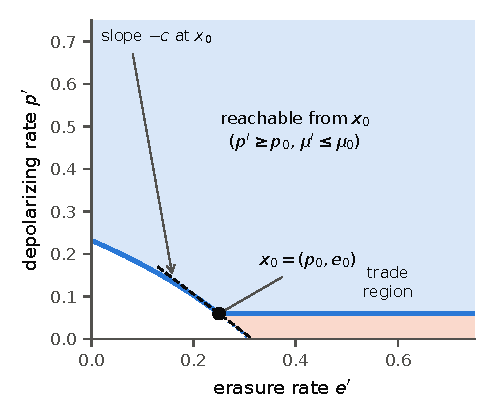
\includegraphics[width=0.48\textwidth]{figures/fig_free_order.pdf}
\caption{The free order seen from $x_0=(p_0,e_0)=(0.06,0.25)$ (computed from Proposition~\ref{prop:two-scalars}). Blue: the points $(p',e')$ reachable by local free operations, bounded by $p'=p_0$ and by the level curve $\mu'=\mu_0$, whose tangent at $x_0$ has slope $-c$ (dashed). Orange: unreachable pairs with more erasure and less Pauli noise; within it lies the trade region of \S\ref{sec:universal}, where the code-universal single-loss order is open.}
\label{fig:free-order}
\end{figure}

\subsection{The uncoded qubit}

Let $\mathfrak D_1$ be one uncoded qubit ($V=\F^2$, no checks, $L=\mathrm{id}$) and $P_{p,e}$ the induced object: with labels $(I,X,Y,Z)$, $P_0=(1-e)(1-p,\tfrac p3,\tfrac p3,\tfrac p3)$ and $P_1=\tfrac e4\mathbf 1$. Its ML failure is $\err=\tfrac34(1-\mu)$.

\begin{proposition}[The uncoded qubit: free order $=$ conditional majorization]\label{prop:local-level1}
For $p,p'\in[0,\tfrac34)$ and $e,e'\in[0,1)$ the following are equivalent: (i) a local free operation maps $\Ncc(p,e)$ to $\Ncc(p',e')$; (ii) $P_{p,e}\red P_{p',e'}$ with arbitrary label permutations; (iii) $\Phi(P_{p',e'})\le\Phi(P_{p,e})$ for all $\varphi\in\Phi_4$.
\end{proposition}
\begin{proof}
(i)$\Rightarrow$(ii) because local free operations are reductions; (ii)$\Leftrightarrow$(iii) is Theorem~\ref{thm:complete}. (ii)$\Rightarrow$(i): let $M$ realize the reduction, $b_a=\sum_{\pi:\pi(I)=a}M(0,\pi\mid0)$, $\tau=\sum_ab_a$ and $y=\sum_\pi M(0,\pi\mid1)$. Then $Q_0=(1-e)\lambda\sum_ab_a\delta_a+c_0\mathbf 1$ and $1-e'=(1-e)\tau+ey$. The output requires $(1-e)\lambda(b_I-b_X)=(1-e')\lambda'$, so $(1-e')\lambda'\le(1-e)\lambda\tau$, and the case analysis of the proof of Theorem~\ref{thm:preorder} applies.
\end{proof}

\subsection{The code-universal order}\label{sec:universal}

Say that $(p,e)\succeq_{\rm univ}(p',e')$ if $\err_{\mathfrak D}(p',e')\ge\err_{\mathfrak D}(p,e)$ for every linear decoding structure $\mathfrak D$ on any number of qubits. By Theorem~\ref{thm:preorder} it contains the free order. A structure \emph{reverses} a pair if $\err_{\mathfrak D}(p',e')<\err_{\mathfrak D}(p,e)$.

\begin{conjecture}[Code-universal order $=$ free order; single loss]\label{conj:universal}
On $\Ncc$, $\succeq_{\rm univ}$ coincides with the free order: every pair that is not related by a local free operation is reversed by some linear decoding structure.
\end{conjecture}

\noindent If $\err$ is replaced by all members of $\Phi_\Lambda$, the statement is true, because the uncoded qubit is one of the structures (Proposition~\ref{prop:local-level1}). The open part is the single loss $\err$, which is what decoder failure rates measure. When all encodings are allowed, ``better for every code'' is characterized by processing orders such as Shannon's inclusion order~\cite{Shannon58} and the equivalence theorems of Buscemi~\cite{Buscemi16,Buscemi18}; the restriction here is to linear structures, the single loss and local operations.

\begin{proposition}[Two structures and a family of monotones]\label{prop:two-structures}
(a) The uncoded qubit has $\err=\tfrac34(1-\mu)$ and reverses exactly the pairs with $\mu'>\mu$.
(b) The two-qubit structure $F_2$ with $S=0$, $N=\langle XX,ZZ\rangle$ (syndrome $E_1+E_2$, label $E_1$) has $\err=p(1-e^2)+\tfrac34e^2=\tfrac34(1-\nu)$ with $\nu=(1-e^2)\lambda(p)$, and reverses exactly the pairs with $\nu'>\nu$.
(c) For every $k\ge1$, $\nu_k=(1-e^k)\lambda(p)$ is a monotone of the free order, and every unreachable pair is separated by some $\nu_k$. The conjecture therefore holds for every unreachable pair with $\mu'>\mu$ or $\nu'>\nu$, in particular for every unreachable pair with $e'<e$.
\end{proposition}
\begin{proof}
(a) $1-\err=(1-e)(1-p)+e/4=\tfrac14+\tfrac34\mu$. (b) Condition on the erased set $A$. For $A=\emptyset$ the two candidate labels at syndrome $s\ne0$ tie, and $1-\err_\emptyset=(1-p)^2+(1-p)p=1-p$; for $|A|=1$, $\err_A=p$; for $|A|=2$, $\err_A=\tfrac34$. (c) Write $\nu_k=\mu\sum_{i<k}e^i$, increasing in $e$ and $\mu$; reachable pairs (Proposition~\ref{prop:two-scalars}) decrease it. An unreachable pair has either $e'<e$ and $\mu'>\mu$, or $e'\ge e$ and $p'<p$, in which case $\nu_k'-\nu_k\to\lambda'-\lambda>0$.
\end{proof}

\noindent The unreachable pairs not covered by (c) with $k\le2$ form the \emph{trade region} $e'\ge e$, $p'<p$, $\mu'\le\mu$, $\nu'\le\nu$: less Pauli noise and more erasure. A structure with $\err_A\approx p$ for all $|A|<k$ (``erasure-hardened of order $k$'') would realize $\nu_k$ to first order and decide the conjecture there. The following obstructions show that such structures do not exist beyond order two (proofs in Appendix~\ref{app:proofs}). Write $\err_A(p)$ for the ML failure with erased set $A$, $V_A$ for the Paulis supported on $A$, and $d_K$ for the smallest weight in $N\setminus S$.

\begin{lemma}[Obstructions]\label{lem:obstructions}
(a) If $G\in N\setminus S$ is supported in $A$, then $\err_A(p)\ge\tfrac12$ for every $p$.
(b) $\err_A(0)=1-2^{-r(A)}$ with $r(A)=\dim(N\cap V_A)-\dim(S\cap V_A)$.
(c) If $\err_\emptyset(p)/p^j\not\to0$ as $p\to0$, then $d_K\le2j$.
\end{lemma}

\begin{corollary}\label{cor:hardening}
If $\err_\emptyset(p)=\Theta(p^j)$, some $A$ with $|A|\le2j$ has $\err_A\ge\tfrac12$, so $\err(p,e)\ge\tfrac12e^{2j}$. No structure that fails at first order in $p$ is erasure-hardened of order $3$.
\end{corollary}

\begin{proposition}[No uniform lower bound on the marginal rate]\label{prop:rate-small-p}
For the Pauli repetition structure $\Rep_k$ ($S=0$, $N=\langle X^{\otimes k},Z^{\otimes k}\rangle$; $\Rep_2=F_2$),
\[
\lim_{p\to0}\frac{R_{\Rep_k}(p,e)}{c(p,e)}=\frac{2e}{2e+(k-1)(1-e)}\qquad(0<e<1),
\]
where $R_{\mathfrak D}=\partial_e\err_{\mathfrak D}/\partial_p\err_{\mathfrak D}$. Hence, at fixed $e_0\in(0,1)$, $\inf_{\mathfrak D}R_{\mathfrak D}(p_0,e_0)/c\to0$ as $p_0\to0$.
\end{proposition}
\begin{proof}
With $m$ non-erased copies the failure is $\tfrac34$ ($m=0$), $p$ ($m=1,2$), and $O(p^2)$ ($m\ge3$, majority vote). Differentiate $\err=\sum_m\binom km(1-e)^me^{k-m}\err_m$ at $p=0$: $\partial_e\err=\tfrac34ke^{k-1}$, $\partial_p\err=k(1-e)e^{k-1}+\binom k2(1-e)^2e^{k-2}$, and $c(0,e)=\tfrac34/(1-e)$.
\end{proof}

\begin{observation}[Search for reversals; evidence on Conjecture~\ref{conj:universal}]\label{obs:search}
An exhaustive enumeration of all linear decoding structures on $n\le3$ qubits (every nested pair $S\le N\le\F^{2n}$; $92{,}881$ structures and $528$ distinct $\err$ tables at $n=3$), with exact ML, together with time-budgeted hill-climbing at $n=4,5,6$, gives the following.
\begin{enumerate}[label=(\alph*)]
\item For six pairs in the trade region, for example $(p,e)=(0.0213,0.05)\to(0,0.25)$ (no Pauli noise at all) and $(0.0213,0)\to(0.015,0.30)$, no structure on $n\le3$ qubits reverses the pair (smallest difference $\err(p',e')-\err(p,e)$ between $+2\times10^{-3}$ and $+1.7\times10^{-2}$), and hill-climbing at $n=4,5$ finds no reversal (smallest ratio $\err(p',e')/\err(p,e)$ between $1.28$ and $3.66$).
\item Just beyond the free-order boundary at $(0.0213,0.2)$, $\Rep_3$ reverses a pair that neither the uncoded qubit nor $F_2$ reverses, so the reversed set is strictly larger than $\{\mu'>\mu\}\cup\{\nu'>\nu\}$.
\item The smallest marginal rate $R_{\mathfrak D}/c$ over $n\le3$ is $0$ at $e_0=0$ (attained by $F_2$, which has $R/c=2e_0/(1+e_0)$ at every $p$), $2e_0/(1+e_0)$ at $e_0\le0.1$, $p_0=0.0213$, and $0.262$ at $(0.0213,0.2)$ ($\Rep_3$); hill-climbing reaches $0.237$ ($n=5$) and $0.235$ ($n=6$) there.
\item For non-degenerate structures ($S=0$), large codes could reverse a pair if a random-coding or expurgated exponent of $(p',e')$ exceeded the sphere-packing exponent of $(p,e)$ at some rate. This sufficient criterion fails for all six trade pairs (the largest gap is between $-0.006$ and $-0.11$ nats).
\end{enumerate}
\end{observation}

\noindent This is evidence that the single-loss form of Conjecture~\ref{conj:universal} \emph{fails} in the trade region, but not a proof: $n\ge7$ is not searched, the hill-climbing at $n\ge4$ is heuristic, and the exponent criterion covers only non-degenerate structures and is only sufficient. If it fails, the code-universal $\err$-order is strictly larger than the free order while the all-losses order equals it; the extra comparabilities would then be a property of the single loss, not evidence of missing free operations.

%=====================================================================
\section{Exchange rates}\label{sec:rates}

\subsection{Definition and the bound}

``Exchange rate'' can mean three different things: (R-a) the \emph{marginal rate} $R_M=\partial_eM/\partial_pM$ of a monotone $M$ at a point; (R-b) a one-shot conversion cost, such as the Pauli equivalent of Corollary~\ref{cor:worth}; (R-c) an asymptotic rate $\sup\{m/n:A^{\otimes n}\red B^{\otimes m}\}$ for independent copies (\S\ref{sec:tensor}). This section concerns (R-a), with $M=\err_d$ (rate $R^{(d)}$), $M=\alpha$ (rate $R_\alpha$; note that $\alpha$ decreases with noise, so $R_\alpha=\partial_e\alpha/\partial_p\alpha$ is a ratio of two negative numbers), or the Bhattacharyya parameter below (rate $R_B$). The suppression exponent of one code family as $d\to\infty$ and the tensor-power limit are different asymptotics.

\begin{theorem}[Partial flag discarding]\label{thm:partial}
For $0\le p\le\tfrac34$, $0\le e_0<1$, $0\le\delta\le1-e_0$, every linear decoding structure on qubits satisfies
\[
\err(p,e_0+\delta)\le\err\big(p+c(p,e_0)\,\delta,\ e_0\big).
\]
Consequently $\alpha_\pm(p,e_0+\delta)\ge\alpha_\pm(p+c\delta,e_0)$ for every code family.
\end{theorem}
\begin{proof}
Apply Lemma~\ref{lem:basic-ops}(c) with $e=e_0+\delta$ and $\kappa=\delta/(e_0+\delta)$: then $e'=e_0$ and $p'=\big((1-e_0-\delta)p+\tfrac34\delta\big)/(1-e_0)=p+\delta(\tfrac34-p)/(1-e_0)$. Apply Theorem~\ref{thm:monotone}.
\end{proof}

\begin{theorem}[Exchange-rate bound]\label{thm:rate}
Let $c=c(p_0,e_0)$.
(a) If $\err$ has right partial derivatives at $(p_0,e_0)$, then $\partial_e\err\le c\,\partial_p\err$; if $\partial_p\err>0$, $R^{(d)}\le c$.
(b) If $\alpha=\alpha_+=\alpha_-$ exists near $(p_0,e_0)$ and has right partial derivatives there with $\partial_p\alpha<0$, then $0\le R_\alpha=\partial_e\alpha/\partial_p\alpha\le c$.
\end{theorem}
\begin{proof}
Subtract the value at $(p_0,e_0)$ from both sides of Theorem~\ref{thm:partial}, divide by $\delta$ and let $\delta\downarrow0$; for $\alpha$ the inequality is reversed and division by $\partial_p\alpha<0$ reverses it again.
\end{proof}

\noindent The bound is a short consequence of partial flag discarding. Three remarks give it content. First, Theorem~\ref{thm:rate-right} removes the differentiability assumption. Second, the bound is sharp in two senses: no better bound follows from the free operations (Proposition~\ref{prop:marginal}), and specific codes attain it (\S\ref{sec:equality}). Third, the familiar heuristic ``an erasure costs $\tfrac34$ of a Pauli error'' is the value at $(0,0)$; in general $c\le\tfrac34$ iff $p_0\ge\tfrac34e_0$, and for example $c(0.02,0.05)=0.768>\tfrac34$. The numerator $\tfrac34-p_0$ reflects that a newly erased qubit already carried Pauli noise of rate $p_0$; the denominator reflects that $p$ is a rate on non-erased qubits.

\begin{proposition}[Marginal rates of the free order]\label{prop:marginal}
Call $M$ a monotone of the free order if $M(p',e')\ge M(p,e)$ whenever $(p,e)$ reaches $(p',e')$. Let $p_0<\tfrac34$, $e_0<1$.
(a) If $M$ has right partial derivatives at $x_0=(p_0,e_0)$, then $\partial_pM\ge0$, $\partial_eM\ge0$ and $\partial_eM\le c\,\partial_pM$.
(b) $p$ and $1-\mu$ are monotones with marginal rates $0$ and $c$; for $a,b\ge0$, $a\,p+b(1-\mu)$ has marginal rate $b\lambda_0/(a+\tfrac43b(1-e_0))$, which takes every value in $[0,c]$.
(c) Hence the set of marginal rates at $x_0$ of monotones of the free order with right partial derivatives is exactly $[0,c]$. In particular $R^{(d)},R_\alpha\in[0,c]$ for every code, and Theorem~\ref{thm:rate} is the sharpest bound that follows from the free operations alone.
\end{proposition}
\begin{proof}
(a) $(p_0,e_0+t)$ reaches $(p_0+ct,e_0)$ with $\mu'=\mu$ (Theorem~\ref{thm:partial}), and $(p_0,e_0)$ reaches $(p_0+t,e_0)$ and $(p_0,e_0+t)$; expand to first order. (b) Monotonicity follows from Proposition~\ref{prop:two-scalars}; $\partial_p(1-\mu)=\tfrac43(1-e_0)$ and $\partial_e(1-\mu)=\lambda_0$, whose ratio is $c$. (c) combines (a) and (b).
\end{proof}

\begin{corollary}[The Pauli equivalent of erasure]\label{cor:worth}
Let $p_{\rm eq}(p,e)=\inf\{p':\err(p',0)\ge\err(p,e)\}$. Then $p\le p_{\rm eq}(p,e)\le p+e(\tfrac34-p)$, the upper bound being Theorem~\ref{thm:partial} with $e_0=0$, $\delta=e$, and the lower bound holding when $\err(\cdot,0)$ is strictly increasing.
\end{corollary}

\subsection{One-sided derivatives}

Fix a structure on $n$ qubits. For an erased set $A$ and rates $q=(q_j)_{j\notin A}$, let $\err_A(q)$ be the ML error when the qubits in $A$ are erased and qubit $j\notin A$ carries $\Dep_{q_j}$. A decision rule $D$ maps syndromes to classes; $L_A(q;D)$ is its failure probability, so $\err_A(q)=\min_DL_A(q;D)$ over finitely many rules, and $\mathcal D^\ast_A(q)$ denotes the set of ML rules.

\begin{lemma}[One qubit]\label{lem:concave}
Fix $A$, $j\notin A$ and the other rates. (a) $q_j\mapsto L_A(q;D)$ is affine on $[0,\tfrac34]$ for every $D$, so $q_j\mapsto\err_A(q)$ is concave. (b) At $q_j=\tfrac34$, $\err_A(q)=\err_{A\cup\{j\}}(q_{-j})$.
\end{lemma}
\begin{proof}
(a) $\Dep_{q_j}$ is affine in $q_j$, hence so are all class weights, and $\err_A=1-\sum_s\max_cW_c$. (b) $\Dep_{3/4}$ is uniform and the position of $j$ is known.
\end{proof}

\begin{lemma}[Danskin form of the envelope identity]\label{lem:danskin}
If every $L(\theta;D)$ is continuous near $\theta^\ast$ and has a one-sided directional derivative in direction $v$, then $\partial^+_v\err(\theta^\ast)=\min_{D\in\mathcal D^\ast(\theta^\ast)}\partial_vL(\theta^\ast;D)$. In particular, if the ML class is unique for every syndrome, the derivative of $\err$ equals the derivative of the failure rate of the decoder frozen at $\theta^\ast$; in general the frozen decoder's derivative is an upper bound on the right derivative.
\end{lemma}
\begin{proof}
A non-ML rule at $\theta^\ast$ stays non-optimal for small $h>0$, so $\err(\theta^\ast+hv)=\min_{D\in\mathcal D^\ast}[\err(\theta^\ast)+h\,\partial_vL(\theta^\ast;D)+o(h)]$.
\end{proof}

\noindent On $\Ncc$ every $L(\cdot;D)$ is a polynomial in $(p,e)$, so the lemma applies in every direction. Moreover the ML decoder depends on $p$ only (the erased positions are observed), so the $e$-derivative of $\err$ needs no envelope argument. This justifies the derivative estimator of \S\ref{sec:numerics}.

\begin{theorem}[Exchange-rate bound with one-sided derivatives]\label{thm:rate-right}
For every linear decoding structure on qubits and every $0\le p<\tfrac34$, $0\le e<1$,
\[
\partial_e\err(p,e)\;\le\;c(p,e)\,\partial_p^+\err(p,e),
\]
where $\partial_e\err$ exists ($\err$ is a polynomial in $e$) and the right derivative $\partial_p^+\err$ exists by Lemma~\ref{lem:danskin}.
\end{theorem}

\noindent The proof (Appendix~\ref{app:proofs}) writes $\partial_e\err$ as a sum of single-qubit increments $\err_{A\cup\{j\}}-\err_A$, bounds each by the right tangent of the concave function of Lemma~\ref{lem:concave} on $[p,\tfrac34]$, and compares the sum of single-qubit right derivatives with the right derivative of the sum by Lemma~\ref{lem:danskin}. The same proof applies to detector error models whose fault locations carry independent depolarizing-plus-erasure noise.

\subsection{When the bound is attained}\label{sec:equality}

\begin{theorem}[Equality criterion]\label{thm:equality}
Let $0<p<\tfrac34$, $0\le e<1$. Then $\partial_e\err=c\,\partial_p^+\err$ iff, for every erased set $A$ of positive probability (only $A=\emptyset$ if $e=0$; all $A$ if $e>0$):
\begin{enumerate}[label=(E\arabic*)]
\item for every $j\notin A$ and every syndrome, some class that is ML-optimal for $(A,p)$ is also ML-optimal when qubit $j$ is erased in addition (\emph{one more flag never changes the ML decision}); and
\item $\min_{D\in\mathcal D^\ast_A}\sum_{j\notin A}\partial_{q_j}L_A(p;D)=\sum_{j\notin A}\min_{D\in\mathcal D^\ast_A}\partial_{q_j}L_A(p;D)$, which holds automatically if the ML class is unique for every syndrome.
\end{enumerate}
In particular, at $e_0=0$ and a rate without ML ties, $R^{(d)}=c$ iff flagging any single qubit leaves an ML decision optimal.
\end{theorem}

\noindent The criterion is a finite statement about ML decisions. At $e_0=0$ it has a polynomial form. Put $r=p/(3(1-p))\in(0,1)$, and for a class $C$ (a coset of $S$ within a syndrome) let $W_C(r)=\sum_{E\in C}r^{\wt E}$ and $W^{(j)}_C(r)=\sum_{E\in C}r^{\wt(E\text{ off }j)}$, where the second weight ignores position $j$.

\begin{proposition}[Polynomial form]\label{prop:lex}
At $e_0=0$, (E1) holds at rate $p$ iff, for every syndrome and qubit $j$, $\arg\max_CW_C(r)\cap\arg\max_CW^{(j)}_C(r)\ne\emptyset$. It holds for all sufficiently small $p$ iff the same is true for the lexicographic order of coefficient sequences read from the lowest power.
\end{proposition}

\noindent Minimum weights never decide (E1) on their own: if $G\in N\setminus S$ has weight $d$ and is split into $E_1E_2$ with disjoint supports of sizes $\lfloor d/2\rfloor$ and $\lceil d/2\rceil$, then $E_1,E_2$ have the same syndrome, lie in different classes whose minimum weights are exactly $\lfloor d/2\rfloor$ and $\lceil d/2\rceil$, and flagging a qubit of $\supp E_2$ equalizes ($d$ odd) or reverses ($d$ even) them. Multiplicities decide instead:

\begin{corollary}[A first-order obstruction]\label{cor:first-order-e1}
Let a syndrome have a unique class $C^\ast$ of minimum weight $w$, let $j$ lie in no weight-$w$ element of $C^\ast$, and let a class $C'\ne C^\ast$ of the same syndrome have minimum weight $w+1$ with
\begin{multline*}
\#\{E\in C':\wt E=w+1,\ j\in\supp E\}\\
>\#\{E\in C^\ast:\wt E=w\}+\#\{E\in C^\ast:\wt E=w+1,\ j\in\supp E\}.
\end{multline*}
Then (E1) fails for all sufficiently small $p$, and $R^{(d)}<c$ there.
\end{corollary}
\begin{proof}
Both flagged polynomials start at $r^w$ with the displayed coefficients, so $C^\ast$ is not a lexicographic maximum after the flag; apply Proposition~\ref{prop:lex} and Theorem~\ref{thm:equality}.
\end{proof}

\begin{proposition}[The five-qubit code attains the bound at every rate]\label{prop:five-hand}
For $[[5,1,3]]$~\cite{LMPZ,BDSW}, with $c^\ast=P_kS$ the class of a single-qubit Pauli $P_k$, $c'$ any nontrivial logical class of the same syndrome, and $j\ne k$, the class polynomials are
\[
\begin{array}{lll}
\text{syndrome }0: & W_S=1+15r^4, & W_{c'}=10r^3+6r^5,\\
& W^{(j)}_S=1+12r^3+3r^4, & W^{(j)}_{c'}=6r^2+4r^3+6r^4,\\
\text{syndrome }\sigma(P_k): & W_{c^\ast}=r+4r^3+8r^4+3r^5, & W_{c'}=2r^2+4r^3+6r^4+4r^5,\\
& W^{(k)}_{c^\ast}=1+12r^3+3r^4, & W^{(k)}_{c'}=6r^2+4r^3+6r^4,\\
& W^{(j)}_{c^\ast}=r+3r^2+7r^3+5r^4, & W^{(j)}_{c'}=r+3r^2+7r^3+5r^4.
\end{array}
\]
The differences are $W_S-W_{c'}=(1-r)^3(1+3r+6r^2)$, $W_{c^\ast}-W_{c'}=r(1-r)^3(1+r)$, $W^{(j)}_S-W^{(j)}_{c'}=W^{(k)}_{c^\ast}-W^{(k)}_{c'}=(1-r)^3(1+3r)$ and $W^{(j)}_{c^\ast}-W^{(j)}_{c'}\equiv0$. Hence for every $p\in(0,\tfrac34)$ the ML class is unique, it stays ML-optimal under any single flag, (E1) and (E2) hold, and $R^{(d)}(p,0)=c(p,0)=\tfrac34-p$.
\end{proposition}

\noindent The proof (Appendix~\ref{app:proofs}) uses only the symmetries of the code. The mechanism is visible in the last row: at a single-error syndrome, flagging any \emph{other} qubit makes all four logical classes exactly equally likely at every $p$, so the flag cannot move the decision; all other flags leave the ML class strictly optimal. The exact uniformity is presumably related to the fact that $[[5,1,3]]$ comes from a perfect tensor (an absolutely maximally entangled (AME) state on six qubits).

\begin{observation}[Other codes]\label{obs:codes}
Exact ML at $e_0=0$ (all $4^n$ errors enumerated) gives the ratios $R^{(d)}/c$ in Table~\ref{tab:codes}. The Steane code~\cite{Steane} satisfies (E1) but has ML ties at $42$ of its $64$ syndromes and fails (E2); the rotated $d=3$ surface code fails (E1); the Shor code also has ties and does not attain the bound. On $300$ random $[[n,1]]$ stabilizer codes ($n=4$--$8$), $10$ attain the bound at all three tested rates; all of them have distance $1$. On $160$ random $[[n,1]]$ codes ($n=4$--$7$), (E1) fails at small $p$ for $138$, and Corollary~\ref{cor:first-order-e1} detects $113$ of these. Among the codes obtained from the stabilizer AME states on $3$, $5$ and $6$ qubits by every choice of $k\ge1$ input legs ($[[2,1,1]]$, $[[4,1,2]]$, $[[3,2,1]]$, $[[5,1,3]]$, $[[4,2,2]]$), all satisfy (E1) at the tested rates $p\in\{10^{-3},0.01,0.05,0.2,0.5\}$, but only $[[5,1,3]]$ has unique ML classes; the others fail (E2) and have $R^{(d)}<c$ (for example $R^{(d)}/c\approx0.80$, $0.75$, $0$ at small $p$ for $[[2,1,1]]$, $[[3,2,1]]$, $[[4,2,2]]$). Qubit AME states exist only for $2,3,5,6$ qubits~\cite{HiguchiSudbery,Scott,HGS}.
\end{observation}

\begin{table}[t]
\centering
\begin{tabular}{lcccc}
\toprule
code & $p=0.02$ & $p=0.06$ & $p=0.15$ & (E1) / unique ML class \\
\midrule
$[[5,1,3]]$ & $1.0000$ & $1.0000$ & $1.0000$ & yes / yes \\
Steane $[[7,1,3]]$ & $0.852$ & $0.841$ & $0.811$ & yes / no \\
Shor $[[9,1,3]]$ & $0.774$ & $0.783$ & $0.804$ & -- / no \\
rotated surface $d=3$ & $0.734$ & $0.734$ & $0.727$ & no / no \\
\bottomrule
\end{tabular}
\caption{Exact $R^{(d)}/c$ at $e_0=0$ (exact enumeration, \texttt{sharp\_codes\_scan.py}; for $[[5,1,3]]$ the ratio equals $1$ to $10^{-14}$ and Proposition~\ref{prop:five-hand} proves equality). The last column is from the tie-aware check K5 (Appendix~\ref{app:checks}); ``--'' means not checked separately.}
\label{tab:codes}
\end{table}

\noindent So neither distance, nor being CSS, nor being a surface code decides equality; for qubits, ``perfect tensor'' explains (E1) on every available example, and $[[5,1,3]]$ is the only one with (E2) as well. A structural description of the codes satisfying (E1) and (E2) is open.

\subsection{The gap is code dependence}

The gap between $c$ and the rate of a particular code cannot be blamed on missing free operations, provided the operations are required to be sound for all codes:

\begin{proposition}[The gap is a property of the code]\label{prop:gap-A}
Let $\succeq$ be any order on $\Ncc$ that contains the free order and under which $\err_{\mathfrak D}$ is monotone for every linear decoding structure $\mathfrak D$ (for example $\succeq_{\rm univ}$). Then the marginal rates at $x_0$ of its monotones that have right partial derivatives lie in $[0,c]$, and $c$ is attained: by the uncoded qubit's $\err=\tfrac34(1-\mu)$, and at $e_0=0$ by $\err$ of $[[5,1,3]]$. In particular no code-universally sound enlargement of the free operations lowers $c$, whether or not Conjecture~\ref{conj:universal} holds, and a strict gap $c-R$ for the surface code is a property of the surface code.
\end{proposition}
\begin{proof}
Monotones of $\succeq$ are monotones of the free order, so Proposition~\ref{prop:marginal}(a) applies; the two attaining monotones are Proposition~\ref{prop:marginal}(b) and Proposition~\ref{prop:five-hand}.
\end{proof}

\noindent What remains is quantitative: where in $[0,c]$ a given code sits. A natural reference is a single-qubit Hellinger monotone. For $s\in(0,1)$ and a shift $G\in V$, $b_s(P;G)=\sum_{E,F}P(E,F)^{1-s}P(E+G,F)^s$ is nondecreasing under (F1), (F2), (F2$'$) (joint concavity of $x^{1-s}y^s$ and translation invariance of convolutions). On $\Ncc$, with a single-qubit shift, its minimum over $s$ is at $s=\tfrac12$:
\[
B(p,e)=e+(1-e)\beta(p),\qquad \beta(p)=2\sqrt{p(1-p)/3}+\tfrac{2p}{3},
\]
the single-qubit Bhattacharyya parameter, which is $\Upsilon(e,p)$ of Dumer, Kovalev and Pryadko~\cite{DKP}. Its marginal rate is $R_B=(1-\beta(p))/\big((1-e)\beta'(p)\big)\le c$. Numerically, the rates of $\Rep_k$ ($k\le7$) approach $R_B$ as $k$ grows at the searched points (for example $R/c=0.268$ for $\Rep_7$ against $R_B/c=0.250$ at $(0.0213,0.05)$). We use $R_B$ only as a reference value in \S\ref{sec:numerics}.

%=====================================================================
\section{Tensor powers of the uncoded qubit}\label{sec:tensor}

The product $P\otimes Q$ of objects is the product law on labels and observations; reductions are compatible with it, and $1-\err(P\otimes Q)=(1-\err(P))(1-\err(Q))$. For the uncoded qubit we can compute the exact and approximate orders on tensor powers. Two functionals are needed. For $\alpha\in\mathbb R\setminus\{0\}$ let $\Phi_\alpha(P)=\sum_y\|P_y\|_\alpha$, and let $g(P)=\max_y\|P_y\|_\infty/\|P_y\|_1$ be the largest posterior probability of a label.

\begin{proposition}[Multiplicative monotones]\label{prop:power-family}
If $P\red Q$ then $\Phi_\alpha(Q)\le\Phi_\alpha(P)$ for $\alpha\in[1,\infty]$, $\Phi_\alpha(Q)\ge\Phi_\alpha(P)$ for $\alpha<1$, $g(Q)\le g(P)$, and $H(L\mid Y)_Q\ge H(L\mid Y)_P$. The functionals $\Phi_\alpha$ and $g$ are multiplicative and $H(L\mid Y)$ is additive under $\otimes$. For the uncoded qubit, $g(P_{p,e})=1-p$, $\Phi_\infty(P_{p,e})=\tfrac14+\tfrac34\mu$ and $H(L\mid Y)=2e+(1-e)H_4(p)$ bits, with $H_4(p)=-(1-p)\log_2(1-p)-p\log_2\frac p3$.
\end{proposition}
\begin{proof}
$\|\cdot\|_\alpha$ ($\alpha\ge1$), $-\|\cdot\|_\alpha$ ($\alpha<1$) and $\varphi_{\rm sh}$ lie in $\Phi_\Lambda$; apply Theorem~\ref{thm:complete}. For $g$, Lemma~\ref{lem:kernel} gives $\|Q_{y'}\|_\infty\le\sum M(y',\pi\mid y)\|P_y\|_\infty\le g(P)\|Q_{y'}\|_1$. The rest is direct.
\end{proof}

\begin{theorem}[Tensor powers and catalysts do not enlarge the order]\label{thm:exact-tensor}
For $p,p'\in[0,\tfrac34)$ and $e,e'\in[0,1)$ the following are equivalent: (i) a local free operation maps $\Ncc(p,e)$ to $\Ncc(p',e')$; (ii) $P_{p,e}^{\otimes n}\red P_{p',e'}^{\otimes n}$ for some $n\ge1$; (iii) $P_{p,e}\otimes C\red P_{p',e'}\otimes C$ for some object $C$.
\end{theorem}
\begin{proof}
(i) implies (ii) and (iii) because reductions tensorize. Conversely, $g$ and $\Phi_\infty$ are monotone and multiplicative with $g(C),\Phi_\infty(C)>0$, so (ii) or (iii) gives $1-p'\le1-p$ and $\mu'\le\mu$, which is Proposition~\ref{prop:two-scalars}.
\end{proof}

\begin{theorem}[Approximate tensor-power conversion]\label{thm:approx-tensor}
Let $P=P_{p,e}$, $Q=P_{p',e'}$ with $e,e'<1$, $p,p'<\tfrac34$, and $h_P=H(L\mid Y)_P$.
(a) If $h_Q>h_P$, there are reductions $P^{\otimes n}\red\widetilde Q_n$ with $\|\widetilde Q_n-Q^{\otimes n}\|_{\rm TV}\to0$.
(b) If $h_Q<h_P$, no sequence of reductions $P^{\otimes n}\red\widetilde Q_n$ has $\|\widetilde Q_n-Q^{\otimes n}\|_{\rm TV}\to0$.
(c) If free uniform labels may be appended so that the alphabets match, the supremum of achievable $\lim m/n$ for approximate conversion $P^{\otimes n}\to Q^{\otimes m}$ is $N(P)/N(Q)$ with $N=2-H(L\mid Y)$ bits.
\end{theorem}

\noindent The proof (Appendix~\ref{app:proofs}) is a conditional typicality argument with Hardy--Littlewood--P\'olya and Birkhoff for (a)~\cite{MarshallOlkin}, and monotonicity plus continuity of conditional entropy for (b). Hence on the uncoded qubit the exact (and catalytic) order is the one-shot order, with boundary slope $c$, whereas the approximate order is the order of $Q_{\rm hash}=1-H(L\mid Y)=1-2e-(1-e)H_4(p)$, with marginal rate
\[
R_{\rm hash}=\frac{2-H_4(p)}{(1-e)\log_2\frac{3(1-p)}{p}}<c.
\]
This is the same dichotomy as majorization versus entropy for pure-state entanglement~\cite{Nielsen}. For example, $(0.0213,0.05)\to(0,0.25)$ is not reachable exactly for any $n$, but $h_P=0.273<h_Q=0.5$ bits, so it is reachable approximately. The approximate order concerns entropy, not guessing: $\err(P^{\otimes n})\to1$.

\paragraph{Relation to large-sample results.}
These two theorems are not, to our knowledge, special cases of the large-sample and catalytic results of Mu et al.~\cite{MPST}, Farooq et al.~\cite{FFHT} or Rubboli et al.~\cite{RHT} (we checked the relevant sections of the full texts). The first two concern Blackwell order and matrix majorization without relabeling. The sufficient conditions for large-sample and catalytic conditional majorization in~\cite[Thm.~6.3]{RHT} are strict inequalities that include a strict support condition (the largest support of a conditional law of the label must be strictly smaller for the input); it fails whenever $p>0$ or $e>0$, since a conditional law then has full support. The rate in~\cite[Thm.~8.1]{RHT} is for exact conversion, and the approximate catalytic result~\cite[Thm.~8.3]{RHT} again assumes a strict support condition. The hard direction of Theorem~\ref{thm:exact-tensor} uses only that two conditional R\'enyi entropies of order $\infty$, $-\log g$ and $-\log\Phi_\infty=H_{\min}(L\mid Y)$, which belong to the family of~\cite{RHT}, are additive monotones; what is specific to the uncoded qubit is that these two already cut out the one-shot order. The rate in Theorem~\ref{thm:approx-tensor}(c) has the same form as the rate between i.i.d.\ pairs in the resource theory of asymmetric distinguishability~\cite{WW19}: $N(P)=D(P\,\|\,u\otimes P_Y)$. For coded structures nothing is proved.

%=====================================================================
\section{Exponents of the surface code}\label{sec:exponents}

We use the rotated surface code of odd distance $d$ on qubits $(r,c)$, $0\le r,c\le d-1$, with plaquettes indexed by their top-left corner $(r,c)$, of $Z$ type iff $r+c$ is odd, weight-$2$ boundary checks, the $Z$ logical on row $0$ and the $X$ logical on column $0$~\cite{BravyiKitaev,DKLP}. Besides $B$ we need $B_M(p,e)=e+(1-e)2\sqrt{q(1-q)}$ with $q=\tfrac23p$, the Bhattacharyya parameter of the $X$ (or $Z$) marginal; it is $\Upsilon_{\rm CSS}(e,q)$ of~\cite{DKP}.

\begin{proposition}[Chernoff upper bound on the exponent]\label{prop:genie}
For $0\le p\le\tfrac34$, $0\le e\le1$, $(p,e)\ne(0,0)$, and every odd $d\ge3$,
\[
\err_d(p,e)\ge\tfrac12B^d\exp\!\big(-\tfrac12\sqrt{d\sigma^2}\big),\qquad\sigma^2=\frac{2(1-e)\sqrt{(1-p)p/3}}{B}\ln^2\frac{3(1-p)}{p}\quad(\sigma^2=0\text{ if }p=0).
\]
Hence $\alpha_+(p,e)\le\ln\frac1{B(p,e)}$.
\end{proposition}

\noindent The proof (Appendix~\ref{app:proofs}) gives the decoder a genie that reveals everything except which of the two classes $E_T$ and $E_T+\bar X_T$ occurred on one interior column $T$; this is a coarse-graining in reverse, so Theorem~\ref{thm:monotone} applies, and the genie's error is a binary hypothesis test between $P_1^{\otimes d}$ and its shift, bounded at finite $d$ through the Bhattacharyya coefficient. For the lower bound on the exponent we use Peierls arguments for a matching decoder, which bound $\err_d$ from above because ML is optimal:

\begin{proposition}[Peierls lower bounds on the exponent]\label{prop:peierls}
Let $\mu_{\rm saw}\approx2.638$ be the connective constant of self-avoiding walks on $\mathbb Z^2$~\cite{MS}. Then $\alpha_-(p,e)\ge\ln\frac1{\mu_{\rm saw}B_M}$ whenever $\mu_{\rm saw}B_M<1$, and $\alpha_-(p,e)\ge\ln\frac1{2B_M}-\ln(1+4B_M+16B_M^2)$ whenever $B_M<0.18$. Explicitly, for $B_M<0.18$ and every odd $d\ge3$,
\[
\err_d(p,e)\le\frac{2d\,B_M\big(2B_M(1+4B_M+16B_M^2)\big)^{d-1}}{\tfrac12-2B_M-8B_M^2}.
\]
\end{proposition}

\begin{corollary}[Sandwich]\label{cor:sandwich}
$\ln\frac1{\mu_{\rm saw}B_M}\le\alpha_-\le\alpha_+\le\ln\frac1B$ whenever $\mu_{\rm saw}B_M<1$. At $p=0$, $B=B_M=e$; at $e=0$, $B_M/B\to\sqrt2$ as $p\to0$.
\end{corollary}

\noindent The two sides are functions of different single-qubit quantities, and a sandwich does not constrain derivatives, so it does not bound exchange rates. Along the erasure axis it can be sharpened to the leading order:

\begin{theorem}[Pure-erasure exponent]\label{thm:erasure-exponent}
For the rotated surface code at $p=0$, $0<e<0.18$, and every odd $d\ge3$,
\[
\tfrac18(2e)^d(1-e)^{d-1}\;\le\;\err_d(0,e)\;\le\;\frac{2d\,e\,\big(2e(1+4e+16e^2)\big)^{d-1}}{\tfrac12-2e-8e^2}.
\]
Hence $\ln\frac1e-\ln2-\ln(1+4e+16e^2)\le\alpha_-(0,e)\le\alpha_+(0,e)\le\ln\frac1e-\ln2+\ln\frac1{1-e}$, that is, $\alpha(0,e)=\ln\frac1e-\ln2+O(e)$.
\end{theorem}

\noindent The $-\ln2$ is the growth rate of the number of minimum-weight logical operators; the proof (Appendix~\ref{app:proofs}) counts minimum-weight $X$ logicals that are paths with one qubit per row (lower bound, with Lemma~\ref{lem:obstructions}(a)) and crossing paths row by row (upper bound, with Lemma~\ref{lem:obstructions}(b)). The thresholds of~\cite{SBD,Colmenarez} concern the critical point; we did not find this explicit exponent in the literature.

\begin{proposition}[Near the erasure axis]\label{prop:hb-status}
For $B_M<0.18$,
\[
\ln\frac1{2B_M}-\ln(1+4B_M+16B_M^2)\le\alpha_-\le\alpha_+\le\min\Big\{\ln\frac1B,\ \ln\frac1{2e}+\ln\frac1{1-e}\Big\}.
\]
If $p\to0$ faster than $e^2$, both sides equal $\ln\frac1B-\ln2+o(1)$: to leading order, $\alpha$ is a function of $B$ near the erasure axis. At $e=0$ the two sides differ by about $\ln(2\sqrt2)\approx1.04$ as $p\to0$.
\end{proposition}
\begin{proof}
Lower side: Proposition~\ref{prop:peierls}. Upper side: Proposition~\ref{prop:genie}, and $\err_d(p,e)\ge\err_d(0,e)$ (adding depolarizing noise on unflagged qubits is free) with Theorem~\ref{thm:erasure-exponent}. If $p=o(e^2)$ then $B/e\to1$ and $B_M/e\to1$.
\end{proof}

\noindent This motivates a hypothesis that the numerics of \S\ref{sec:numerics} test:

\begin{conjecture}[Hypothesis $H_B$]\label{conj:HB}
In some neighbourhood in $\Ncc$, the exponent $\alpha(p,e)$ of the rotated surface code is a function of $B(p,e)$, so that $R_\alpha=R_B$.
\end{conjecture}

\noindent A heuristic supports it at small $B$: along both axes the dominant failures (half of a minimum-weight logical in error at $e=0$; a whole minimum-weight logical erased at $p=0$) give $\err_d\approx N_dB^d$ up to factors $e^{o(d)}$, with $N_d$ the number of minimum-weight logicals. A proof at $e=0$ would need a lower bound on $\err_d$ that captures the entropy of minimum-weight logicals, which the single-column genie misses, and an upper bound for a decoder that uses $X$--$Z$ correlations, so that the per-qubit factor is $B$ rather than $B_M$. The domain-wall reading of $\alpha$~\cite{DKLP,CF} and path-entropy analyses at low error rates~\cite{WatsonBarrett,BBKM,English} are the relevant framework.

%=====================================================================
\section{Surface-code exchange rates: numerics}\label{sec:numerics}

\paragraph{Method.}
We estimate $\pL(d)=\err_d$ and its derivatives for the rotated surface code at six work points $p_0\in\{0.04,0.06\}$, $e_0\in\{0,0.02,0.05\}$, $d=5,7,9,11$ (and $13$), with the Bayes-optimal decoder matched to $(p_0,e_0)$: an exact transfer-matrix coset decoder for $d\le11$ and a truncated matrix-product-state decoder (bond dimension $8$ with a refinement monitor) at $d=13$, both supporting per-qubit priors (uniform on erased qubits), in the spirit of~\cite{BSV}. The estimator is stratified by the number $k$ of erased qubits and the number $w$ of Pauli errors: $\pL=\sum_{k,w}P_{p,e}(k,w)f(k,w)$ with exactly known binomial weights and Monte Carlo estimates of the stratum failure fractions $f$, which vanish when $2w+k<d$; samples are allocated by Neyman allocation. Derivatives come from differentiating the weights at fixed $f$: for $e$ this is exact (the ML decoder does not depend on $e$), and for $p$ it is the frozen-decoder derivative, which equals $\partial_p\err$ whenever the ML decision is unique (Lemma~\ref{lem:danskin}). Errors are from a parametric bootstrap ($500$ replicates). The exponent $\alpha$ and its derivatives come from inverse-variance weighted least-squares fits of $\ln\pL(d)$ and $\partial\ln\pL(d)$ against $d$ over a window (default $d=5$--$11$), and $R_\alpha=\partial_e\alpha/\partial_p\alpha$. The decoders were validated against exhaustive enumeration at $d=3$, against an independent MPS implementation at $d=3,5$, and the frozen-decoder derivative against re-matched finite differences at $d=5,7,9$ (Appendix~\ref{app:checks}).

\begin{table}[t]
\centering
\small
\begin{tabular}{cccccccccc}
\toprule
$p_0$ & $e_0$ & $c$ & $R^{(5)}$ & $R^{(7)}$ & $R^{(9)}$ & $R^{(11)}$ & $R_\alpha$ ($d=5$--$11$) & $R_\alpha/c$ & $R_B$\\
\midrule
0.06 & 0    & 0.690 & 0.387(29) & 0.289(37) & 0.382(70) & 0.209(121) & 0.15(12) & 0.22 & 0.244\\
0.06 & 0.02 & 0.704 & 0.323(14) & 0.273(14) & 0.282(20) & 0.257(34) & 0.204(38) & 0.29 & 0.249\\
0.06 & 0.05 & 0.726 & 0.308(10) & 0.294(10) & 0.260(13) & 0.278(18) & 0.239(25) & 0.33 & 0.257\\
0.04 & 0    & 0.710 & 0.313(25) & 0.431(48) & 0.384(99) & 0.251(137) & 0.53(13) & 0.74 & 0.221\\
0.04 & 0.02 & 0.724 & 0.300(13) & 0.237(14) & 0.270(29) & 0.311(47) & 0.195(47) & 0.27 & 0.226\\
0.04 & 0.05 & 0.747 & 0.264(8) & 0.265(11) & 0.252(18) & 0.231(23) & 0.233(28) & 0.31 & 0.233\\
\bottomrule
\end{tabular}
\caption{Marginal exchange rates of the rotated surface code with ML decoding (from \texttt{results/p1\_exchange\_rate.json}; standard errors in units of the last digits). $R^{(d)}=\partial_e\pL/\partial_p\pL$; $R_\alpha$ from weighted fits over $d=5$--$11$; $c$ is the bound of Theorem~\ref{thm:rate}; $R_B$ is the Bhattacharyya reference.}
\label{tab:surface}
\end{table}

\begin{figure}[t]
\centering
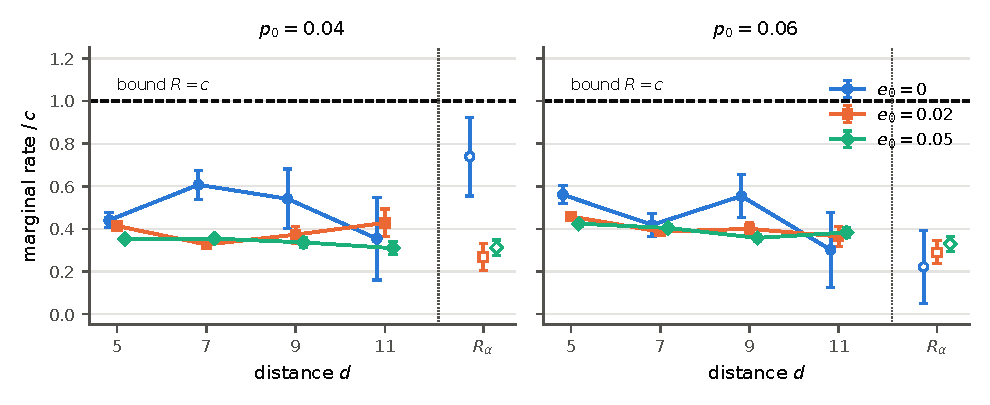
\includegraphics[width=\textwidth]{figures/fig_surface_rates.pdf}
\caption{Finite-distance marginal rates $R^{(d)}/c$ of the rotated surface code with ML decoding at $p_0=0.04$ (left) and $0.06$ (right), $e_0\in\{0,0.02,0.05\}$ (colours and markers; points slightly offset horizontally), with one-standard-error bars; open markers at the right: the exponent rate $R_\alpha/c$ (fit window $d=5$--$11$). Dashed: the bound $R=c$. Data: \texttt{results/p1\_exchange\_rate.json}.}
\label{fig:surface}
\end{figure}

\begin{observation}[Surface-code exchange rates]\label{obs:surface}
Table~\ref{tab:surface} and Figure~\ref{fig:surface}:
\begin{enumerate}[label=(\alph*)]
\item $R^{(d)}\le c$ at every point with a large margin: $R^{(d)}/c$ lies between about $0.31$ and $0.61$ for $d\le11$.
\item At $e_0=0.02$ and $0.05$, $R_\alpha=0.195$--$0.239$, i.e.\ $R_\alpha/c\approx0.27$--$0.33$: an erasure is worth about a third of what the flag-discarding bound allows, and $c-R_\alpha\approx0.5$.
\item At these four points $R_\alpha$ agrees with $R_B$ within about one standard error (ratios $R_\alpha/R_B$ between $0.82$ and $1.00$). Hypothesis $H_B$ is consistent with the data, but not confirmed.
\item At $e_0=0$ the estimates are poor: $\partial_e\pL$ at $e=0$ is a difference between the strata with one erasure and none, with large variance, and $R_\alpha$ is window-dependent (Table~\ref{tab:window}). These points carry no information beyond $R^{(d)}\le c$.
\end{enumerate}
\end{observation}

\begin{table}[t]
\centering
\small
\begin{tabular}{ccccccc}
\toprule
$p_0$ & $e_0$ & $d=5$--$9$ & $d=5$--$11$ & $d=7$--$11$ & $d=5$--$13$ & $R_B$\\
\midrule
0.06 & 0    & 0.18(13) & 0.15(12) & 0.37(27) & 0.15(12) & 0.244\\
0.06 & 0.02 & 0.201(43) & 0.204(38) & 0.266(80) & 0.199(40) & 0.249\\
0.06 & 0.05 & 0.224(29) & 0.239(25) & 0.225(49) & 0.251(27) & 0.257\\
0.04 & 0    & 0.63(15) & 0.53(13) & 0.06(34) & 0.53(13) & 0.221\\
0.04 & 0.02 & 0.146(51) & 0.195(47) & 0.411(138) & 0.219(50) & 0.226\\
0.04 & 0.05 & 0.250(34) & 0.233(28) & 0.184(90) & 0.243(31) & 0.233\\
\bottomrule
\end{tabular}
\caption{Fit-window dependence of $R_\alpha$ (weighted fits). The $d=13$ points carry relative errors of $54$--$870\%$ in $\pL$ and almost no weight.}
\label{tab:window}
\end{table}

\paragraph{Systematics and caveats.}
(1) \emph{Fit window.} At $(0.04,0.02)$ the rate moves from $0.146$ ($d=5$--$9$) to $0.411$ ($d=7$--$11$), about $1.8$ combined standard errors; at the two $e_0=0.05$ points the windows agree within errors. The quoted $R_\alpha$ is therefore a finite-size estimate on $d\le11$, not an asymptotic value. (2) \emph{Distance range.} ML at $d=13$ was too expensive at the required precision (the dominant ML failure fractions are small; $10\%$ relative error at $d=13$ would need $10^6$--$10^7$ decodes per point), and $p_0=0.02$ was not run. (3) \emph{Envelope identity.} The frozen-decoder $p$-derivative was tested against re-matched finite differences for the exact decoder up to $d=9$; for the MPS decoder only its decisions were validated. (4) \emph{Code capacity only.} Nothing here is measured at circuit level.

\paragraph{Matching.} For comparison, MWPM (with $X$ and $Z$ decoded separately and erased qubits at weight $0$) on $d=5$--$21$ gives, on the window $d=5$--$11$, exponents smaller than ML by $\Delta\alpha=0.19$--$0.27$ and $R_\alpha^{\rm MWPM}=0.16$--$0.19$ at $e_0>0$; at $e_0=0$ its finite-$d$ rates for $d\le13$ are $0.66$--$0.88$, around and partly above $c$. This does not contradict Theorem~\ref{thm:rate}: MWPM is not Bayes-optimal and is not matched to $(p,e)$ (Remark~\ref{rem:ml-only}). The MWPM exponents drift with the window (for example $0.249\to0.300$ at $(0.06,0.02)$ from $d=5$--$11$ to $d=11$--$21$), so $\Delta\alpha$ carries a systematic error beyond its statistical one.

\paragraph{Reading.} The surface code sits at $R_\alpha/c\approx0.3$, close to where the large repetition structures $\Rep_k$ and $R_B$ sit ($R_B/c\approx0.31$--$0.35$ at $p_0=0.04$--$0.06$). By Proposition~\ref{prop:gap-A}, this gap is a property of the surface code. As an independent, purely heuristic comparison: the secant of the threshold curve between the depolarizing ML threshold $p_c\approx0.189$~\cite{Bombin} (computed for the toric code) and the erasure threshold $e_c=0.5$~\cite{SBD} has slope $0.38$, well below $c\approx0.75$; at threshold, Corollary~\ref{cor:worth} requires only $e_c\ge\tfrac43p_c\approx0.25$.

%=====================================================================
\section{Related work}\label{sec:related}

\paragraph{Comparison of experiments and conditional majorization.}
Simulation of one decision problem by another goes back to Blackwell~\cite{Blackwell} and is the subject of Torgersen's monograph~\cite{Torgersen}; quantum versions are due to Buscemi~\cite{Buscemi12}, Matsumoto~\cite{Matsumoto}, Chefles~\cite{Chefles} and Jen\v{c}ov\'a~\cite{Jencova}. With relabeling of a classical label given classical side information, the order is the conditional majorization of Gour et al.~\cite{GGHKLN}; Brandsen, Geng and Gour~\cite{BGG} construct games of chance inducing it, and Rubboli, Haapasalo and Tomamichel~\cite{RHT} characterize conditional entropies through it and study its large-sample and catalytic forms. Large-sample Blackwell order and matrix majorization are treated in~\cite{MPST,FFHT}. Resource theories whose order is a majorization-type order are reviewed in~\cite{ChitambarGour}, with entanglement~\cite{Nielsen} and thermodynamics~\cite{GMNSH} as prototypes. For channels, ``better for every code'' corresponds to processing orders~\cite{Shannon58,Buscemi16,Buscemi18}.

\paragraph{Channel resource theories and distinguishability.}
Noise is a channel, and (F1)--(F2$'$) are restricted superchannels~\cite{CDP08,CDP09} that use the flags but not the hidden fault. General resource theories of channels are set up in~\cite{LiuWinter,GourScandolo}; Gour~\cite{Gour19} compares channels under superchannels via an extended conditional min-entropy. The resource of the theory of asymmetric distinguishability of Wang and Wilde~\cite{WW19,WW19ch} is closely related: a reduction maps the pair $(P,u\otimes P_Y)$ to $(Q,u\otimes Q_Y)$, so their monotones give necessary conditions for our order. For two labels without relabeling, the order is decided by relative Lorenz curves~\cite{BuscemiGour}. That discrimination tasks are complete tests is known for general convex resource theories~\cite{TakagiRegula} and for channel transformations~\cite{RBL}. The resource theory of coding of Wang, Liu, Wang and Luo~\cite{WLWL} orders codes, not noise models.

\paragraph{Erasure versus Pauli noise.}
The value of erasures has been quantified through thresholds and logical error rates~\cite{SBD,WKPT,Sahay,KubicaErasure,Chang,GRK,GVRK}, and the combinatorial rule $2w+k\le d-1$ is classical~\cite{GBP}. Classical analogues of a two-scalar order are the extremality results for binary erasure and symmetric channels of Hirche and Shaya~\cite{HircheShaya} and contraction-based orders of quantum channels~\cite{HRSF}; flagged depolarizing channels are used to bound capacities in~\cite{FKG}. We did not find an analytic exchange-rate bound such as Theorem~\ref{thm:rate}, an equality criterion such as Theorem~\ref{thm:equality}, or a characterization of the free order such as Theorem~\ref{thm:preorder}.

\paragraph{Exponents.}
The parameters $B$ and $B_M$ appear in the threshold bounds for degenerate LDPC codes of Dumer, Kovalev and Pryadko~\cite{DKP} (see also~\cite{KovalevPryadko,KPDP}); the Peierls argument is that of~\cite{DKLP}. The domain-wall reading of $\alpha$ is due to~\cite{DKLP,CF}; path entropy at low error rates is analysed in~\cite{WatsonBarrett,BBKM}, and an effective tension model in~\cite{English}. Erasure and computational errors are treated together via the coherent information in~\cite{Colmenarez}. The depolarizing ML threshold of the toric code is $18.9(3)\%$~\cite{Bombin}. ML decoding of the surface code by tensor networks is due to Bravyi, Suchara and Vargo~\cite{BSV}, and erasure decoding in linear time to Delfosse and Z\'emor~\cite{DZ}.

%=====================================================================
\section{Open problems}\label{sec:open}

\begin{enumerate}[leftmargin=2em]
\item \emph{The single-loss code-universal order} (Conjecture~\ref{conj:universal}). Decide whether some linear structure reverses a pair in the trade region. The search evidence (Observation~\ref{obs:search}) points to a negative answer; a proof would need control of the exponent curves $R\mapsto E(R;P)$ for degenerate structures, not a single R\'enyi parameter.
\item \emph{Lower bounds on exchange rates.} By Proposition~\ref{prop:rate-small-p}, no lower bound on $\inf_{\mathfrak D}R_{\mathfrak D}$ is uniform in $p_0$; whether it is positive at each fixed $p_0>0$, $e_0>0$ is a question about large structures. For the surface code, a rigorous lower bound on $R_\alpha$ is open.
\item \emph{Hypothesis $H_B$ at $e=0$.} Prove $\alpha=\ln\frac1B-\lim\frac1d\ln N_d+o(1)$ as $p\to0$; this needs a lower bound on $\err_d$ that sees path entropy and a correlated-decoder Peierls bound with per-qubit factor $B$.
\item \emph{Codes attaining the bound.} Characterize the codes satisfying (E1) and (E2); prove that every AME code satisfies (E1); treat qudits.
\item \emph{Coded tensor powers.} Extend Theorems~\ref{thm:exact-tensor} and~\ref{thm:approx-tensor} beyond the uncoded qubit.
\item \emph{Numerics.} Exact or certified ML exchange rates beyond $d=11$, at $p_0=0.02$, and at circuit level, where Theorem~\ref{thm:rate-right} still applies to the detector error model with independent depolarizing-plus-erasure faults.
\end{enumerate}

\paragraph{Acknowledgements.} [To be added.]

%=====================================================================
\appendix

\section{Proofs}\label{app:proofs}

\subsection{Lemma~\ref{lem:obstructions} and Corollary~\ref{cor:hardening}}
(a) Given $A$, the fault is uniform on $A$, so $P_A(E+G)=P_A(E)$. Since $G\in N$ the syndrome is unchanged and since $G\notin S$ the class $E+S$ moves to a different class of the same syndrome with the same weight; so every best class has an equally likely twin, and the success probability is at most $\tfrac12$.
(b) At $p=0$ the fault is uniform on $V_A$. Its syndromes correspond to the cosets of $N\cap V_A$ in $V_A$, and within one syndrome the classes are cosets of $S\cap V_A$, all of the same size; so there are $2^{r(A)}$ equally likely classes.
(c) If $d_K>2j$, two faults of weight $\le j$ with the same syndrome differ by an element of $N$ of weight $\le2j$, which lies in $S$; so at each syndrome all faults of weight $\le j$ lie in one class $C_0$ and every other class has weight $O(p^{j+1})$, while $W(C_0)\ge(p/3)^j(1-p)^n$. For small $p$, $C_0$ wins and $\err_\emptyset=O(p^{j+1})$.
Corollary~\ref{cor:hardening}: by (c) some $G\in N\setminus S$ has weight $\le2j$; take $A=\supp G$ in (a).

\subsection{Theorem~\ref{thm:rate-right}}
Write $\pi_A=e^{|A|}(1-e)^{n-|A|}$, so $\err(p,e)=\sum_A\pi_A\err_A(p)$. (1) Reindexing $B=A\cup\{j\}$ and using $\pi_{B\setminus\{j\}}=\pi_B(1-e)/e$,
\[
\partial_e\err=\frac1{1-e}\sum_A\pi_A\sum_{j\notin A}\big[\err_{A\cup\{j\}}(p)-\err_A(p)\big]
\]
(at $e=0$ only $A=\emptyset$ contributes). (2) Let $f_{A,j}(q)$ be $\err_A$ with qubit $j$ at rate $q$ and the others at $p$. By Lemma~\ref{lem:concave}, $\err_{A\cup\{j\}}(p)-\err_A(p)=f_{A,j}(\tfrac34)-f_{A,j}(p)\le(\tfrac34-p)f_{A,j}'^{\,+}(p)$. (3) By Lemma~\ref{lem:danskin}, $f_{A,j}'^{\,+}(p)=\min_{D\in\mathcal D^\ast_A}\partial_{q_j}L_A(p;D)$ and $\partial_p^+\err_A(p)=\min_{D\in\mathcal D^\ast_A}\sum_{j\notin A}\partial_{q_j}L_A(p;D)\ge\sum_{j\notin A}f_{A,j}'^{\,+}(p)$. Combining, $\partial_e\err\le c\sum_A\pi_A\partial_p^+\err_A(p)=c\,\partial_p^+\err$.

\subsection{Theorem~\ref{thm:equality} and Proposition~\ref{prop:lex}}
Equality in Theorem~\ref{thm:rate-right} holds iff it holds in step (2) for every $(A,j)$ with $\pi_A>0$ and in step (3) for every such $A$; the latter is (E2). In (2), a concave function meets its right tangent at $\tfrac34$ iff it is affine on $[p,\tfrac34]$. Now $f_{A,j}=1-\sum_sg_s$ with $g_s=\max_CW_C$ convex, and a sum of convex functions is affine iff each summand is. $g_s$ is affine on $[p,\tfrac34]$ iff some class is maximal at both endpoints: if $W_C$ is maximal at both ends, every $W_{C'}-W_C$ is affine and $\le0$ at both ends; conversely, a class maximal at an interior point coincides with the affine $g_s$ on the whole segment. Maximality at $q_j=p$ is ML-optimality for $(A,p)$, and at $q_j=\tfrac34$ ML-optimality for $A\cup\{j\}$ (Lemma~\ref{lem:concave}(b)); this is (E1).
For Proposition~\ref{prop:lex}: $\Prob[C]=(1-p)^nW_C(r)$ and, with $j$ erased, $\tfrac14(1-p)^{n-1}W^{(j)}_C(r)$; common factors do not affect maximizers, and $f(r)>g(r)$ for all small $r>0$ iff the coefficient sequence of $f$ is lexicographically larger.

\subsection{Proposition~\ref{prop:five-hand}}
Facts. (a) $S$ is generated by the cyclic shifts of $XZZXI$; its $15$ nontrivial elements have weight $4$, and $N\setminus S$ has weight distribution $30x^3+18x^5$. (b) The cyclic shift and the transversal map $X\to Y\to Z\to X$ preserve $S$; the shift fixes each logical class and the transversal map permutes the three nontrivial ones, so each nontrivial class has $10$ elements of weight $3$ and $6$ of weight $5$, and $3$ stabilizers miss each qubit. (c) For a qubit $m$, the stabilizers missing $m$ form with $I$ a group of order $4$ whose nontrivial elements have weight $4$, so at every other qubit they take the values $X,Y,Z$ once each. Restriction to qubit $k$ is a homomorphism $S\to\F^2$ with kernel of order $4$, so every value at $k$ occurs $4$ times in $S$ and in every class $LS$. (d) Two distinct elements of a class differ by a stabilizer, so their product has weight $\ge4$.

The class $c'=P_kLS$ consists of $P_kL'$, $L'\in LS$. By (c), $L'_k=I$ for $4$ elements, which have weight $3$. For a value $Q\ne I$ at $k$, two weight-$3$ elements with $L'_k=Q$ have a product of weight $\le4$ supported off $k$, so by (d) their other two qubits form complementary pairs among the four qubits $\ne k$; hence at most $2$ per value, and since $6$ weight-$3$ elements have $L'_k\ne I$, exactly $2$ per value, and then (c) gives exactly $2$ weight-$5$ elements per value. By (d), the four weight-$3$ elements with $L'_k=I$ have distinct supports. In $c^\ast=P_kS$: $P_k$ itself; for each $m\ne k$ exactly one stabilizer with $s_k=P_k$ missing $m$, giving weight $3$; $8$ stabilizers with $s_k\notin\{I,P_k\}$, two missing each $m\ne k$, giving weight $4$; and $3$ stabilizers missing $k$, giving weight $5$. Reading off the weights and the weights off $j$ or off $k$ gives the table; for syndrome $0$ use that $6$ of the $10$ weight-$3$ elements of a class contain a given qubit and $12$ of the $15$ stabilizers do. The factorizations follow by expansion. All differences are $\ge0$ on $(0,1)$, strictly for the unflagged ones; apply Proposition~\ref{prop:lex} at every $p$ and Theorem~\ref{thm:equality}. (Check H1 recomputes the table for all $16$ syndromes and all single flags, and K5 certifies the conclusion in exact integer arithmetic; Appendix~\ref{app:checks}.)

\subsection{Theorem~\ref{thm:approx-tensor}}
(a) For a flag string $y\in\{0,1\}^n$ with $m(y)$ unflagged positions, $P^{\otimes n}_y=\Prob_P(y)\,s_y$ with $s_y=\Dep_p^{\otimes\text{unflagged}}\otimes u^{\otimes\text{flagged}}$; likewise $t_{y'}$ for $Q$. Fix $\delta$ with $4\delta<h_Q-h_P$ and let $Y_n,Y_n'$ be the flag strings with $|m(y)-(1-e)n|\le n^{2/3}$ (resp.\ $e'$). For $y\in Y_n$, $-\log s_y(X)$ is a sum of $m(y)$ i.i.d.\ terms of mean $H_4(p)$ plus $2(n-m(y))$, so by Chebyshev $B_y=\{x:s_y(x)\ge2^{-n(h_P+\delta)}\}$ has $s_y(B_y^c)\le\epsilon_n\to0$ uniformly; likewise $A_{y'}=\{x:t_{y'}(x)\le2^{-n(h_Q-\delta)}\}$ has $t_{y'}(A_{y'}^c)\le\epsilon_n$. Let $\tilde t_{y'}=(1-2\epsilon_n)t_{y'}\mathbf 1_{A_{y'}}/t_{y'}(A_{y'})+2\epsilon_nu_{\Lambda^n}$, so $\|\tilde t_{y'}-t_{y'}\|_{\rm TV}\le4\epsilon_n$. For large $n$, $\tilde t_{y'}$ is majorized by $s_y$: for $k\le|B_y|$ the $k$ largest entries of $\tilde t$ sum to at most $2k\,2^{-n(h_Q-\delta)}\le k\,2^{-n(h_P+\delta)}$; for $k>|B_y|$ the $4^n-k$ smallest entries of $\tilde t$ sum to at least $(4^n-k)2\epsilon_n4^{-n}$ and those of $s_y$ to at most $(4^n-k)\epsilon_n/(4^n-|B_y|)$, with $|B_y|\le4^n/2$. By Hardy--Littlewood--P\'olya and Birkhoff~\cite{MarshallOlkin}, $\tilde t_{y'}$ is a mixture of permutations of $s_y$. The kernel $M(y',\pi\mid y)=\Prob_Q(y')w_{yy'}(\pi)$, with these Birkhoff weights for $y\in Y_n$, $y'\in Y_n'$ and uniform weights otherwise, produces $\widetilde Q_n$ within $\Prob_P(Y_n^c)+\Prob_Q(Y_n'^c)+4\epsilon_n\to0$ of $Q^{\otimes n}$.
(b) $H(L\mid Y)$ is monotone and additive, so $H(L\mid Y)_{\widetilde Q_n}\ge nh_P$; by continuity of entropy~\cite[Thm.~17.3.3]{CT} on alphabets of size $8^n$ and $2^n$, $|H(L\mid Y)_{\widetilde Q_n}-nh_Q|=o(n)$ when the distance tends to $0$, so $h_Q\ge h_P$.
(c) The padded objects have conditional entropies $nh_P+2(k-n)$ and $mh_Q+2(k-m)$; apply (a) and (b).

\subsection{Proposition~\ref{prop:genie}}
Take the $d$ qubits $T$ of an interior column $c_0$ ($1\le c_0\le d-2$) and the $X$-type operator $\bar X_T$ on it. \emph{Step 1: $\ker\sigma\cap V_T=\{I,\bar X_T\}$ and $\bar X_T\notin S$.} For each $r\le d-2$ the two bulk plaquettes with corners $(r,c_0-1)$, $(r,c_0)$ have opposite types and meet $T$ in $\{(r,c_0),(r+1,c_0)\}$, which forces the $X$ part and the $Z$ part of a syndrome-free $E$ on $T$ to be constant along the column; the weight-$2$ $X$-type boundary check on the top edge that contains $(0,c_0)$ meets $T$ only there, which forces the $Z$ part to vanish. $\bar X_T$ has zero syndrome and anticommutes with the $Z$ logical on row $0$. \emph{Step 2.} A genie that reveals $F$, $E_{T^c}$ and $\sigma(E)$ leaves only the binary question $E_T\in\{a,a+\bar X_T\}$, with different labels; the real observation is a coarse-graining of the genie's, so $\err_d\ge\varepsilon_{\rm genie}=\tfrac12(1-\mathrm{TV}(P_1^{\otimes d},Q_1^{\otimes d}))$, where $P_1$ is the law of one qubit's $(a,f)$ and $Q_1=P_1(\cdot+X)$. \emph{Step 3.} With $\Lambda=\ln(P/Q)$, $\min(P,Q)=\sqrt{PQ}\,e^{-|\Lambda|/2}$ and $\sum\sqrt{PQ}=B^d$, so $\varepsilon_{\rm genie}=\tfrac12B^d\E_R[e^{-|\Lambda|/2}]$ with $R=\sqrt{PQ}/B^d$ a product law under which $\Lambda$ is a sum of $d$ i.i.d.\ symmetric terms of variance $\sigma^2$ (flagged qubits and $a\in\{Y,Z\}$ contribute $0$; $a\in\{I,X\}$ unflagged contribute $\pm\ln\frac{3(1-p)}p$). Jensen and Cauchy--Schwarz give $\E_Re^{-|\Lambda|/2}\ge e^{-\sqrt{d\sigma^2}/2}$. At flagged positions the two hypotheses coincide, which is the origin of the $e$ in $B$.

\subsection{Proposition~\ref{prop:peierls} and Theorem~\ref{thm:erasure-exponent}}
\emph{Peierls bound~\cite{DKLP}.} Decode the $X$ and $Z$ parts separately by a minimum-weight correction, where weight counts non-erased qubits. For the $X$ part, form the graph whose vertices are the $Z$ checks and a boundary vertex, with qubit $j$ as an edge. On failure, $E\oplus C$ contains a simple cycle through the boundary vertex with odd overlap with the $Z$ logical on row $0$, which is a crossing path $\gamma$ of qubits from row $0$ to row $d-1$ (consecutive qubits sharing a $Z$ check), and minimality forces at least half of the non-erased qubits of $\gamma$ to carry an $X$ error. The $X$ components of non-erased qubits are independent Bernoulli($q$), $q=\tfrac23p$, so the probability of this event for a fixed $\gamma$ is at most $B_M^{|\gamma|}$ (Chernoff with $t=(1-q)/q$). Hence $\err_d\le\pL^{\rm MWPM}\le2\sum_\gamma B_M^{|\gamma|}$, the $2$ accounting for the $Z$ part.
\emph{Counting.} (i) The $Z$-check graph is a subgraph of a square lattice in rotated coordinates, so there are at most $2d\,c_{\ell-2}$ crossing paths of $\ell$ qubits, with $c_m$ the number of $m$-step self-avoiding walks on $\mathbb Z^2$; submultiplicativity~\cite{MS} gives $\alpha_-\ge\ln\frac1{\mu_{\rm saw}B_M}$. (ii) Classify each step of a path by its change of row ($+1,0,-1$); from a qubit there are at most $2$ continuations of each kind, a path of $\ell$ qubits has net displacement $d-1$, and it starts at one of $d$ qubits. Dropping simplicity, for any $\tau>0$, $\sum_\gamma x^{|\gamma|}\le d\,x\sum_{L\ge d-1}(xf(\tau))^L\tau^{-(d-1)}$ with $f(\tau)=2\tau+2+2/\tau$; with $\tau=1/(4x)$, $xf(\tau)=\tfrac12+2x+8x^2$ and
\[
\sum_\gamma x^{|\gamma|}\le\frac{d\,x\,\big(2x(1+4x+16x^2)\big)^{d-1}}{\tfrac12-2x-8x^2}\qquad(0<x<0.18).
\]
With $x=B_M$ this gives the explicit bound of Proposition~\ref{prop:peierls}.
\emph{Theorem~\ref{thm:erasure-exponent}, upper bound.} By Lemma~\ref{lem:obstructions}(b), $\err_d(0,e)\le\Prob[r(A)\ge1]$; a nontrivial logical supported on $A$ has a nontrivial $X$ or $Z$ part whose support contains a crossing path, so $\Prob[r(A)\ge1]\le2\sum_\gamma e^{|\gamma|}$; use the display with $x=e$.
\emph{Lower bound.} A minimum-weight $X$ logical can be a path with one qubit per row: from $(r,c)$ the next qubit is $(r+1,c)$ or the diagonal neighbour sharing the $Z$ check of $(r,c)$ towards row $r+1$. Let $\Gamma$ be the paths starting at the centre of row $0$ with at most $\frac{d-1}2$ diagonal moves; they stay in the lattice and $|\Gamma|\ge2^{d-2}$. Order $\Gamma$ by the first row where two paths differ, left first; if $\gamma'\prec\gamma$ then $\gamma'$ contains a qubit of the set $N_L(\gamma)$ of left alternatives along $\gamma$ ($|N_L(\gamma)|\le d-1$, disjoint from $\gamma$). With $A$ the erased set,
\[
\Prob\Big[\bigcup_{\gamma\in\Gamma}\{\gamma\subseteq A\}\Big]\ge\sum_\gamma\Prob[\gamma\subseteq A]\,\Prob[A\cap N_L(\gamma)=\emptyset]\ge2^{d-2}e^d(1-e)^{d-1},
\]
and on this event $\err_A\ge\tfrac12$ by Lemma~\ref{lem:obstructions}(a).

\section{Computer-assisted checks}\label{app:checks}
\sloppy

All checks are in the repository (\texttt{theory/checks/}). The scripts \texttt{exact\_small\_codes.py}, \texttt{constitution.py}, \texttt{handproof\_checks.py} and \texttt{completion\_checks.py} were rerun while preparing this paper and all their checks passed; the search results and the remaining checks are quoted from the stored outputs in \texttt{results/}. Exact enumeration means summing over all $4^n$ Paulis (and all erased sets) in floating point unless stated otherwise.
\begin{itemize}[leftmargin=1.5em]
\item \emph{K5} (\texttt{completion\_checks.py}): exact integer-polynomial certificate that the ML decision of $[[5,1,3]]$ is unique and unchanged by any single flag for all $0<p<\tfrac34$; tie-aware tests that (E1) fails for the $d=3$ rotated surface code and holds for Steane with non-unique ML classes. \emph{H1} (\texttt{handproof\_checks.py}): the class-polynomial table of Proposition~\ref{prop:five-hand} for all $16$ syndromes and all single flags, and the factorizations.
\item \emph{C3, C4, C7, C8} (\texttt{exact\_small\_codes.py}): partial flag discarding, monotonicity under the free order, $R^{(d)}\le c$, and the envelope identity to relative $2\times10^{-10}$, on $[[5,1,3]]$, Steane and the $d=3$ surface code.
\item \emph{N1} (\texttt{constitution.py}): linear-programming feasibility of $P_{p,e}\red P_{p',e'}$ agrees with Theorem~\ref{thm:preorder}(ii) on a grid (Proposition~\ref{prop:local-level1}); N2--N6 test Theorem~\ref{thm:complete} and the structural properties on random objects.
\item \emph{K1, K2} (\texttt{completion\_checks.py}): the geometry of Step 1 of Proposition~\ref{prop:genie} for every interior column, $d=3$--$41$, over $\F$; the finite-$d$ genie bound against exact $\varepsilon_{\rm genie}$ for $d\le61$.
\item \emph{Searches}: \texttt{universal\_order\_search.py} and \texttt{hardened\_structures\_search.py} (Observation~\ref{obs:search}; exhaustive for $n\le3$, heuristic hill-climbing beyond, not bit-reproducible), \texttt{exponent\_criterion.py}, \texttt{sharp\_codes\_scan.py} (Table~\ref{tab:codes}), \texttt{second\_pass\_checks.py} (L1, Corollary~\ref{cor:first-order-e1}) and \texttt{third\_pass\_checks.py} (M3, M8: tensor-power example and AME codes).
\item \emph{Decoders}: transfer-matrix ML versus brute force at $d=3$ with erasures (agreement to $10^{-15}$); stratified ML versus exact oracle; an independent MPS decoder (qecsim) at $d=3,5$; truncated MPS versus exact decisions at $d=11,13$ ($\chi\ge6$ at $e=0$, $\chi\ge8$ with erasures: no changed decisions); frozen versus re-matched derivatives at $d=5,7,9$ (largest deviation $2.05$ standard errors, $0.1\%$ of the derivative).
\end{itemize}
No interval arithmetic is used in this paper; the only certificate in exact arithmetic is K5.

\section{Reproducibility and correspondence with the source notes}\label{app:repro}

The statements are taken from the theory notes \texttt{theory/main.tex} of the repository; Table~\ref{tab:map} lists the correspondence. Figures are produced by \texttt{papers/exchange-rates/figures/make\_figures.py} from \texttt{results/p1\_exchange\_rate.json} (commit \texttt{37d5819}, \texttt{git\_dirty\_src} false), which was generated by \texttt{experiments/p1\_erasure\_pauli/p1\_exchange\_rate.py analyze} from the stratified tables in \texttt{results/p1\_m2/tables/}; the MWPM comparison is \texttt{results/p1\_mwpm\_margin.json}.

\begin{table}[h]
\centering
\footnotesize
\begin{tabular}{ll@{\quad}ll}
\toprule
here & notes & here & notes\\
\midrule
Thm.~\ref{thm:monotone} & Thm.~1.7 & Thm.~\ref{thm:equality} & Thm.~3.31\\
Lem.~\ref{lem:basic-ops} & Lem.~2.5 & Prop.~\ref{prop:lex} & Prop.~3.33\\
Lem.~\ref{lem:kernel}, Thm.~\ref{thm:complete} & Lem.~0.2, Thm.~0.6 & Cor.~\ref{cor:first-order-e1} & Cor.~3.35\\
Thm.~\ref{thm:preorder}, Prop.~\ref{prop:two-scalars} & Thm.~3.7, Prop.~3.15 & Prop.~\ref{prop:five-hand} & Props.~3.32, 3.36\\
Prop.~\ref{prop:local-level1} & Prop.~0.9 & Obs.~\ref{obs:codes} & Obs.~3.5, 3.38, Prop.~3.32\\
Conj.~\ref{conj:universal} & Conj.~3.11 & Prop.~\ref{prop:gap-A} & Prop.~3.37\\
Prop.~\ref{prop:two-structures} & Prop.~3.16 & Prop.~\ref{prop:power-family} & Props.~0.12, 0.13\\
Lem.~\ref{lem:obstructions}, Cor.~\ref{cor:hardening} & Lems.~3.19--3.21, Cor.~3.22 & Thms.~\ref{thm:exact-tensor}, \ref{thm:approx-tensor} & Thms.~0.14, 0.15\\
Prop.~\ref{prop:rate-small-p} & Prop.~3.23 & Prop.~\ref{prop:genie} & Prop.~5.1\\
Obs.~\ref{obs:search} & Obs.~3.17, 3.24, Rem.~3.25 & Prop.~\ref{prop:peierls} & Prop.~5.2(c), Thm.~4.15,\\ & & & Prop.~4.22, Lem.~5.15\\
Thms.~\ref{thm:partial}, \ref{thm:rate} & Thms.~3.1, 3.2 & Cor.~\ref{cor:sandwich} & Cor.~5.3\\
Prop.~\ref{prop:marginal} & Prop.~0.11 & Thm.~\ref{thm:erasure-exponent} & Thm.~5.16\\
Cor.~\ref{cor:worth} & Cor.~3.4 & Prop.~\ref{prop:hb-status} & Prop.~5.17\\
Lems.~\ref{lem:concave}, \ref{lem:danskin} & Lems.~3.28, 3.29 & Conj.~\ref{conj:HB} & Conj.~3.12\\
Thm.~\ref{thm:rate-right} & Thm.~3.30 & Obs.~\ref{obs:surface} & Obs.~3.26\\
\bottomrule
\end{tabular}
\caption{Correspondence between this paper and the theory notes (numbering of \texttt{theory/main.pdf} at commit \texttt{ae6c92c}).}
\label{tab:map}
\end{table}

% References. Entries marked [notes] are copied verbatim from theory/main.tex (checked there against arXiv/Crossref);
% entries marked [new] were checked against their arXiv abstract pages and Crossref on 2026-10-04.
\begin{thebibliography}{99}
\bibitem{WKPT} Y.~Wu, S.~Kolkowitz, S.~Puri, J.~D.~Thompson, \emph{Erasure conversion for fault-tolerant quantum computing in alkaline earth Rydberg atom arrays}, Nat.\ Commun.\ 13, 4657 (2022), arXiv:2201.03540. % [notes]
\bibitem{KubicaErasure} A.~Kubica, A.~Haim, Y.~Vaknin, F.~Brand\~ao, A.~Retzker, \emph{Erasure qubits: overcoming the $T_1$ limit in superconducting circuits}, Phys.\ Rev.\ X 13, 041022 (2023), arXiv:2208.05461. % [notes]
\bibitem{Sahay} K.~Sahay, J.~Jin, J.~Claes, J.~D.~Thompson, S.~Puri, \emph{High threshold codes for neutral atom qubits with biased erasure errors}, Phys.\ Rev.\ X 13, 041013 (2023), arXiv:2302.03063. % [notes]
\bibitem{SBD} T.~M.~Stace, S.~D.~Barrett, A.~C.~Doherty, \emph{Thresholds for topological codes in the presence of loss}, Phys.\ Rev.\ Lett.\ 102, 200501 (2009), arXiv:0904.3556. % [notes]
\bibitem{GBP} M.~Grassl, T.~Beth, T.~Pellizzari, \emph{Codes for the quantum erasure channel}, Phys.\ Rev.\ A 56, 33 (1997), arXiv:quant-ph/9610042. % [new]
\bibitem{GRK} S.~Gu, A.~Retzker, A.~Kubica, \emph{Fault-tolerant quantum architectures based on erasure qubits}, Phys.\ Rev.\ Research 7, 013249 (2025), arXiv:2312.14060. % [notes]
\bibitem{GVRK} S.~Gu, Y.~Vaknin, A.~Retzker, A.~Kubica, \emph{Optimizing quantum error correction protocols with erasure qubits}, PRX Quantum 6, 040354 (2025), arXiv:2408.00829. % [notes]
\bibitem{Chang} K.~Chang, S.~Singh, J.~Claes, K.~Sahay, J.~Teoh, S.~Puri, \emph{Surface code with imperfect erasure checks}, PRX Quantum 6, 040355 (2025), arXiv:2408.00842. % [notes]
\bibitem{GGHKLN} G.~Gour, A.~Grudka, M.~Horodecki, W.~K\l{}obus, J.~\L{}odyga, V.~Narasimhachar, \emph{The conditional uncertainty principle}, Phys.\ Rev.\ A 97, 042130 (2018), arXiv:1506.07124. % [notes]
\bibitem{Blackwell} D.~Blackwell, \emph{Equivalent comparisons of experiments}, Ann.\ Math.\ Stat.\ 24, 265 (1953). % [notes]
\bibitem{Torgersen} E.~Torgersen, \emph{Comparison of Statistical Experiments}, Cambridge University Press (1991). % [notes]
\bibitem{RHT} R.~Rubboli, E.~Haapasalo, M.~Tomamichel, \emph{A complete characterisation of conditional entropies}, arXiv:2601.23213 (2026). % [notes]
\bibitem{Buscemi12} F.~Buscemi, \emph{Comparison of quantum statistical models: equivalent conditions for sufficiency}, Commun.\ Math.\ Phys.\ 310, 625 (2012), arXiv:1004.3794. % [notes]
\bibitem{Buscemi16} F.~Buscemi, \emph{Degradable channels, less noisy channels, and quantum statistical morphisms: an equivalence relation}, Probl.\ Inf.\ Transm.\ 52, 201 (2016), arXiv:1511.08893. % [notes]
\bibitem{Buscemi18} F.~Buscemi, \emph{Comparison of noisy channels and reverse data-processing theorems}, in Proc.\ 2017 IEEE Information Theory Workshop (ITW), pp.~489--493 (2017), arXiv:1803.02945. % [notes]
\bibitem{BGG} S.~Brandsen, I.~J.~Geng, G.~Gour, \emph{What is entropy? A perspective from games of chance}, Phys.\ Rev.\ E 105, 024117 (2022), arXiv:2103.08681. % [notes]
\bibitem{DKP} I.~Dumer, A.~A.~Kovalev, L.~P.~Pryadko, \emph{Thresholds for correcting errors, erasures, and faulty syndrome measurements in degenerate quantum codes}, Phys.\ Rev.\ Lett.\ 115, 050502 (2015), arXiv:1412.6172. % [notes]
\bibitem{Pryadko} L.~P.~Pryadko, \emph{On maximum-likelihood decoding with circuit-level errors}, Quantum 4, 304 (2020), arXiv:1909.06732. % [notes]
\bibitem{DKLP} E.~Dennis, A.~Kitaev, A.~Landahl, J.~Preskill, \emph{Topological quantum memory}, J.\ Math.\ Phys.\ 43, 4452 (2002). % [notes]
\bibitem{IyerPoulin} P.~Iyer, D.~Poulin, \emph{Hardness of decoding quantum stabilizer codes}, IEEE Trans.\ Inf.\ Theory 61, 5209 (2015), arXiv:1310.3235. % [notes]
\bibitem{BSV} S.~Bravyi, M.~Suchara, A.~Vargo, \emph{Efficient algorithms for maximum likelihood decoding in the surface code}, Phys.\ Rev.\ A 90, 032326 (2014). % [notes]
\bibitem{KRS} R.~K\"onig, R.~Renner, C.~Schaffner, \emph{The operational meaning of min- and max-entropy}, IEEE Trans.\ Inf.\ Theory 55, 4337 (2009), arXiv:0807.1338. % [new]
\bibitem{TakagiRegula} R.~Takagi, B.~Regula, \emph{General resource theories in quantum mechanics and beyond: operational characterization via discrimination tasks}, Phys.\ Rev.\ X 9, 031053 (2019), arXiv:1901.08127. % [notes]
\bibitem{RBL} D.~Rosset, F.~Buscemi, Y.-C.~Liang, \emph{Resource theory of quantum memories and their faithful verification with minimal assumptions}, Phys.\ Rev.\ X 8, 021033 (2018), arXiv:1710.04710. % [notes]
\bibitem{Shannon58} C.~E.~Shannon, \emph{A note on a partial ordering for communication channels}, Inf.\ Control 1, 390 (1958). % [notes]
\bibitem{LMPZ} R.~Laflamme, C.~Miquel, J.~P.~Paz, W.~H.~Zurek, \emph{Perfect quantum error correcting code}, Phys.\ Rev.\ Lett.\ 77, 198 (1996), arXiv:quant-ph/9602019. % [new]
\bibitem{BDSW} C.~H.~Bennett, D.~P.~DiVincenzo, J.~A.~Smolin, W.~K.~Wootters, \emph{Mixed-state entanglement and quantum error correction}, Phys.\ Rev.\ A 54, 3824 (1996), arXiv:quant-ph/9604024. % [new]
\bibitem{Steane} A.~M.~Steane, \emph{Multiple-particle interference and quantum error correction}, Proc.\ R.\ Soc.\ Lond.\ A 452, 2551 (1996), arXiv:quant-ph/9601029. % [new]
\bibitem{HiguchiSudbery} A.~Higuchi, A.~Sudbery, \emph{How entangled can two couples get?}, Phys.\ Lett.\ A 273, 213 (2000), arXiv:quant-ph/0005013. % [new]
\bibitem{Scott} A.~J.~Scott, \emph{Multipartite entanglement, quantum-error-correcting codes, and entangling power of quantum evolutions}, Phys.\ Rev.\ A 69, 052330 (2004), arXiv:quant-ph/0310137. % [new]
\bibitem{HGS} F.~Huber, O.~G\"uhne, J.~Siewert, \emph{Absolutely maximally entangled states of seven qubits do not exist}, Phys.\ Rev.\ Lett.\ 118, 200502 (2017), arXiv:1608.06228. % [new]
\bibitem{MarshallOlkin} A.~W.~Marshall, I.~Olkin, B.~C.~Arnold, \emph{Inequalities: Theory of Majorization and Its Applications}, 2nd ed., Springer (2011). % [new]
\bibitem{Nielsen} M.~A.~Nielsen, \emph{Conditions for a class of entanglement transformations}, Phys.\ Rev.\ Lett.\ 83, 436 (1999), arXiv:quant-ph/9811053. % [notes]
\bibitem{MPST} X.~Mu, L.~Pomatto, P.~Strack, O.~Tamuz, \emph{From Blackwell dominance in large samples to R\'enyi divergences and back again}, Econometrica 89, 475 (2021). % [notes]
\bibitem{FFHT} M.~U.~Farooq, T.~Fritz, E.~Haapasalo, M.~Tomamichel, \emph{Matrix majorization in large samples}, IEEE Trans.\ Inf.\ Theory 70, 3118 (2024), arXiv:2301.07353. % [notes]
\bibitem{WW19} X.~Wang, M.~M.~Wilde, \emph{Resource theory of asymmetric distinguishability}, Phys.\ Rev.\ Research 1, 033170 (2019), arXiv:1905.11629. % [notes]
\bibitem{BravyiKitaev} S.~B.~Bravyi, A.~Yu.~Kitaev, \emph{Quantum codes on a lattice with boundary}, arXiv:quant-ph/9811052 (1998). % [new]
\bibitem{MS} N.~Madras, G.~Slade, \emph{The Self-Avoiding Walk}, Birkh\"auser (1993) (submultiplicativity, Ch.~1; exact counts $c_n$ of square-lattice walks are tabulated there and in OEIS A001411). % [notes]
\bibitem{Colmenarez} L.~Colmenarez, S.~Kim, M.~M\"uller, \emph{Fundamental thresholds for computational and erasure errors via the coherent information}, PRX Quantum 6, 040327 (2025), arXiv:2412.16727. % [notes]
\bibitem{CF} C.~T.~Chubb, S.~T.~Flammia, \emph{Statistical mechanical models for quantum codes with correlated noise}, Ann.\ Inst.\ Henri Poincar\'e D 8, 269 (2021). % [notes]
\bibitem{WatsonBarrett} F.~H.~E.~Watson, S.~D.~Barrett, \emph{Logical error rate scaling of the toric code}, New J.\ Phys.\ 16, 093045 (2014), arXiv:1312.5213. % [notes]
\bibitem{BBKM} M.~E.~Beverland, B.~J.~Brown, M.~J.~Kastoryano, Q.~Marolleau, \emph{The role of entropy in topological quantum error correction}, J.\ Stat.\ Mech.\ (2019) 073404, arXiv:1812.05117. % [notes]
\bibitem{English} L.~H.~English, S.~Roberts, S.~D.~Bartlett, A.~C.~Doherty, D.~J.~Williamson, \emph{Ising on the donut: regimes of topological quantum error correction from statistical mechanics}, PRX Quantum (2026), doi:10.1103/4wvz-1p8m, arXiv:2512.10399. % [notes]
\bibitem{Bombin} H.~Bombin, R.~S.~Andrist, M.~Ohzeki, H.~G.~Katzgraber, M.~A.~Martin-Delgado, \emph{Strong resilience of topological codes to depolarization}, Phys.\ Rev.\ X 2, 021004 (2012), arXiv:1202.1852. % [new]
\bibitem{Matsumoto} K.~Matsumoto, \emph{A quantum version of randomization criterion}, arXiv:1012.2650 (2010). % [notes]
\bibitem{Chefles} A.~Chefles, \emph{The quantum Blackwell theorem and minimum error state discrimination}, arXiv:0907.0866 (2009). % [notes]
\bibitem{Jencova} A.~Jen\v{c}ov\'a, \emph{Comparison of quantum channels and statistical experiments}, arXiv:1512.07016 (2015). % [notes]
\bibitem{ChitambarGour} E.~Chitambar, G.~Gour, \emph{Quantum resource theories}, Rev.\ Mod.\ Phys.\ 91, 025001 (2019), arXiv:1806.06107. % [notes]
\bibitem{GMNSH} G.~Gour, M.~P.~M\"uller, V.~Narasimhachar, R.~W.~Spekkens, N.~Yunger Halpern, \emph{The resource theory of informational nonequilibrium in thermodynamics}, Phys.\ Rep.\ 583, 1 (2015), arXiv:1309.6586. % [notes]
\bibitem{CDP08} G.~Chiribella, G.~M.~D'Ariano, P.~Perinotti, \emph{Transforming quantum operations: quantum supermaps}, EPL 83, 30004 (2008), arXiv:0804.0180. % [notes]
\bibitem{CDP09} G.~Chiribella, G.~M.~D'Ariano, P.~Perinotti, \emph{Theoretical framework for quantum networks}, Phys.\ Rev.\ A 80, 022339 (2009), arXiv:0904.4483. % [notes]
\bibitem{LiuWinter} Z.-W.~Liu, A.~Winter, \emph{Resource theories of quantum channels and the universal role of resource erasure}, arXiv:1904.04201 (2019). % [notes]
\bibitem{GourScandolo} G.~Gour, C.~M.~Scandolo, \emph{Dynamical resources}, arXiv:2101.01552 (2020). % [notes]
\bibitem{Gour19} G.~Gour, \emph{Comparison of quantum channels by superchannels}, IEEE Trans.\ Inf.\ Theory 65, 5880 (2019), arXiv:1808.02607. % [notes]
\bibitem{WW19ch} X.~Wang, M.~M.~Wilde, \emph{Resource theory of asymmetric distinguishability for quantum channels}, Phys.\ Rev.\ Research 1, 033169 (2019), arXiv:1907.06306. % [notes]
\bibitem{BuscemiGour} F.~Buscemi, G.~Gour, \emph{Quantum relative Lorenz curves}, Phys.\ Rev.\ A 95, 012110 (2017), arXiv:1607.05735. % [notes]
\bibitem{WLWL} D.-S.~Wang, Y.-D.~Liu, Y.-J.~Wang, S.~Luo, \emph{Quantum resource theory of coding for error correction}, Phys.\ Rev.\ A 110, 032413 (2024), arXiv:2409.09416. % [notes]
\bibitem{HircheShaya} C.~Hirche, O.~Shaya, \emph{Partial orders and contraction for BISO channels}, arXiv:2504.16726 (2025). % [notes]
\bibitem{HRSF} C.~Hirche, C.~Rouz\'e, D.~Stilck Fran\c{c}a, \emph{On contraction coefficients, partial orders and approximation of capacities for quantum channels}, Quantum 6, 862 (2022), arXiv:2011.05949. % [notes]
\bibitem{FKG} M.~Fanizza, F.~Kianvash, V.~Giovannetti, \emph{Quantum flags, and new bounds on the quantum capacity of the depolarizing channel}, Phys.\ Rev.\ Lett.\ 125, 020503 (2020), arXiv:1911.01977. % [notes]
\bibitem{KovalevPryadko} A.~A.~Kovalev, L.~P.~Pryadko, \emph{Fault tolerance of ``bad'' quantum low-density parity check codes}, Phys.\ Rev.\ A 87, 020304(R) (2013), arXiv:1208.2317. % [notes]
\bibitem{KPDP} A.~A.~Kovalev, S.~Prabhakar, I.~Dumer, L.~P.~Pryadko, \emph{Numerical and analytical bounds on threshold error rates for hypergraph-product codes}, Phys.\ Rev.\ A 97, 062320 (2018), arXiv:1804.01950. % [notes]
\bibitem{DZ} N.~Delfosse, G.~Z\'emor, \emph{Linear-time maximum likelihood decoding of surface codes over the quantum erasure channel}, Phys.\ Rev.\ Research 2, 033042 (2020). % [notes]
\bibitem{CT} T.~Cover, J.~Thomas, \emph{Elements of Information Theory}, 2nd ed., Wiley (2006), Ch.~11. % [notes]
\end{thebibliography}


\end{document}
